\documentclass[11pt,a4paper]{book}

\usepackage{lib/Textbook} 
\exhyphenpenalty=10000\hyphenpenalty=10000
%\sloppy
\usepackage{enumitem}
\usepackage{mdframed}
\usepackage{tikz}
\usepackage{nccmath}
\usepackage{wrapfig}
\usepackage{textcomp}
\usepackage{multirow}
\usepackage{tasks}
\usetikzlibrary{shapes,arrows,decorations.pathreplacing,calc,positioning,intersections}
\usepackage[export]{adjustbox}
\usepackage{chngcntr}
\usepackage{array}
\usepackage{picture}
\tikzstyle{Box} = [rectangle, minimum height=1cm, draw=black]
\tikzstyle{arrow} = [thick, ->, >=stealth]

\newlist{steps}{enumerate}{1}
\setlist[steps, 1]{label = Step \arabic*:}

\newcommand{\R}{\mathbb{R}}
\newcommand{\N}{\mathbb{N}}
\newcommand{\Z}{\mathbb{Z}}
\newcommand{\Q}{\mathbb{Q}}
\newcommand{\W}{\mathbb{W}}
\newcommand{\C}{\mathbb{C}}

\usepackage{ulem}
\usepackage{graphicx}

\usepackage[english]{babel}
\usepackage{lipsum}
\usepackage{xcolor}
\usepackage{tikz}
\usepackage{mathtools,amsfonts,amssymb,amsthm}
\usepackage[most]{tcolorbox}
\setlength{\parindent}{0pt}

\usepackage{fourier}




\let\cleardoublepage=\clearpage


% Start document
\begin{document}

\tableofcontents

\chapter{Permutations and Combinations}
\section{Basic Counting Principles}

Is a password with at least one uppercase letter really more secure
than one without? What are my odds of winning the lottery? How many
ways could I arrange my friends around the dining table at my dinner
party? In everyday life, we often need to \textquotedblleft count\textquotedblright{}
the number of ways to arrange objects. However listing out all the
possible arrangements is not always easy. In this chapter we will
be learning some fundamental counting techniques, to help us answer
some of life's burning questions. 

\subsection{Addition Principle for Counting}

\begin{tcolorbox}[colback=blue!5, colframe=black, boxrule=.4pt, sharpish corners]

The \textbf{Addition Principle for Counting} states that if we have
$a_{1}$ ways of doing something and $a_{2}$ ways of doing another
thing and we cannot do both at the same time, then the number of ways
we can choose $a_{1}$ \textbf{or} $a_{2}$ is 
\[
a_{1}+a_{2}
\]
\end{tcolorbox}

Zoe is trying to decide what to wear to the prom. She has 2 ball gowns,
3 blouses and 1 sundress. 

How many different outfits can Zoe choose from? 

Zoe has $2+3+1=6$ outfits to choose from.

\subsection{Multiplication Principle for Counting}

\begin{tcolorbox}[colback=blue!5, colframe=black, boxrule=.4pt, sharpish corners]

The \textbf{Multiplication Principle for Counting} states that if
there is a sequence of independent events that can occur $a_{1},a_{2},a_{3},...a_{n}$
ways, then the number of ways all the events can occur is 
\[
a_{1}\times a_{2}\times a_{3}\times\ldots\times a_{n}
\]
\end{tcolorbox}

Suppose there are three towns $A$, $B$ and $C$ and that four different
roads can be taken from $A$ to $B$ and two different roads from
$B$ to $C$.
\begin{center}
\includegraphics[width=8cm]{\string"../../../../Creative Cloud Files/CountingProductRule\string".png}
\par\end{center}

This begs the question: ``How many different pathways are there from
$A$ to $C$, going through $B$?''

\begin{minipage}[t]{0.5\textwidth} 

If we take road 1, there are two different roads to complete our trip.\\

If we take road 2, there are two different roads to complete our trip
... etc.\\

\end{minipage}
\begin{minipage}[t]{0.2\textwidth} 
\begin{center}
\includegraphics[width=8cm]{\string"../../../../Creative Cloud Files/CountingProductRule1\string".png}
\par\end{center}

\end{minipage}

So there are $2+2+2+2=4\times2$ different pathways we can take from
$A$ to $C$.

\newpage

Similarly, for 
\begin{center}
\includegraphics[width=12cm]{\string"../../../../Creative Cloud Files/CountingProductRule2\string".png}
\par\end{center}

There would be $4\times2\times3=24$ different pathways from $A$
to $D$, passing through $B$ and $C$.

\section{Permutations }

Lisa invites six guests to her birthday party: Raj, Alice, Jerry,
Michelle, Ryan and Heather. When they arrive, they shake hands with
each other. Jerry asks: ``How many handshakes happened in total?''

\textquotedblleft I shook 6 hands altogether\textquotedblright{} says
Ryan, ``and I guess, so did everybody else.''

\textquotedblleft Since there are seven of us, this should mean $7\cdot6=42$
handshakes in total!'' ventures Michelle.

\textquotedblleft This seems too many\textquotedblright{} says Heather.
``The same logic gives 2 handshakes if two persons meet, which is
clearly wrong.\textquotedblright{}

\textquotedblleft That is because every handshake was counted twice.
We have to divide $42$ by $2$, to get the right number: $21$.\textquotedblright{}
settles Lisa the issue.

Lisa and her guests make their way to the dining table to eat. Since
it is Lisa's birthday, she sits at the head of the table. How many
different seatings are there (with Lisa\textquoteright s place fixed)? 

\medskip

\centerline{\begin{minipage}{.68\textwidth} 
\begin{tcolorbox}[colback=blue!5, colframe=black, boxrule=.4pt, sharpish corners]

A \textbf{permutation} is an \textbf{ordered arrangement} of a number
of objects.
\end{tcolorbox}
\end{minipage}}

\medskip{}

Let us fill the seats one by one, starting with the chair on Lisa's
right. There are $6$ choices for the guest who will sit down first.
How many choices are there for the guest who goes second? There are
only $5$ choices as the person who went first is already seated.
Therefore there are a total of $6\cdot5$ ways to seat the first two
guests. 

We can then proceed in a similar manner: we have $4$ choices for
the third guest to be seated, $3$ choices for the fourth guest to
be seated, and so on. Therefore, the number of ways in which the guests can be seated is
\[
6\cdot5\cdot4\cdot3\cdot2\cdot1=6!=720
\]

\centerline{\begin{minipage}{.58\textwidth}  
\begin{tcolorbox}[colback=blue!5, colframe=black, boxrule=.4pt, sharpish corners]

The number of permutations of $n$ different objects is $n!$
\end{tcolorbox}

\end{minipage}}

\begin{example}[Seven Layer Cake]

Alice made a seven layer rainbow cake for Lisa. How many ways could
she have arranged the layers of the cake with the $7$ distinct colours
of the rainbow?

\Solution

The answer is $7!=5040$. 

\end{example}

The simplicity of the answer to the this question was due to several
factors: we used each of our objects exactly once, the order of the
objects mattered, and the objects were all different. In the rest
of this section we will study problems without one or more of these
simplifying factors. 

\subsection{Permutations Involving Identical Objects}

\begin{example}[Flowers in a Row (Repeated Colours)]

A gardener has five red flowers, three yellow flowers and two white
flowers to plant in a row. In how many different ways can she do that?

\Solution

This problem differs from the previous one in only one aspect: the
objects are not all different. We are going to answer this question
by reducing it to the previous one, in which all objects were different.
Assume our gardener plants her flowers in a row, then sticks labels
(say numbers 1 through 5 for the red flowers, 1 through 3 for the
yellow ones, and 1 through 2 for the white ones) to her flowers so
that she can distinguish them. Now she has ten different flowers,
and therefore the row of flowers she has just finished working on
can look $10!$ different ways. We have to tell how many of these
arrangements differ only because of these labels.

The five red flowers could be given five different labels in $5!$
different ways. The three yellow flowers could be given three different
labels in $3!$ different ways. The two white flowers could be given
two different labels in $2!$ different ways. Therefore, the labeling
of all ten flowers can be done in $5!\cdot3!\cdot2!$ different ways.
Therefore, the total number of arrangements when the labels are removed
is
\[
\frac{10!}{5!\cdot3!\cdot2!}=2520
\]

\end{example}


\medskip{}

\begin{tcolorbox}[colback=blue!5, colframe=black, boxrule=.4pt, sharpish corners]

The number of permutations of $n$ objects with $n_{1}$ identical
objects of the first type, $n_{2}$ identical objects of the second
type, ..., and $n_{k}$ identical objects of the $k$ type is 
\[
\frac{n!}{n_{1}!n_{2}!\ldots n_{k}!}
\]
\end{tcolorbox}


\subsection{Permutations Involving Non-Identical Objects}

\subsubsection{Non-Identical Objects Taken Without Repetition}

\begin{example}[20 Politicians Filling 5 Position]

A president must choose five politicians from a pool of 20 candidates
to fill five different cabinet positions. In how many different ways
can she do that?

\Solution

Indeed, we have $20$ choices for the first candidate, $19$ choices
for the second, and so on, just as we did the case of factorials.
The only difference is that here we do not have $20$ slots to fill.
We stop after choosing $5$ of them. 

The number $20\cdot19\cdot18\cdot17\cdot16$ is denoted by $^{20}P_{5}$.
Thus, there are $^{20}P_{5}=1860480$ ways of filling this cabinet.
If the candidates are all equally qualified, it may take a while.

\end{example}

\medskip{}

\begin{tcolorbox}[colback=blue!5, colframe=black, boxrule=.4pt, sharpish corners]

The number of permutations of $n$ different objects taken $r$ at
a time \textbf{without repetition} is 
\[
^{n}P_{r}=\frac{n!}{\left(n-r\right)!}
\]
\end{tcolorbox}


\subsubsection{Non-Identical Objects Taken With Repetition}

\begin{example}[Building 10 Intersections]

A city has recently built ten intersections. Some of these will get
traffic lights, and some of those that get traffic lights will also
get a gas station. In how many different ways can this happen?

\Solution

For each intersection, there are three possible scenarios:

\begin{enumerate}

\item  No traffic light and no gas station.

\item  Traffic light but no gas station.

\item  Traffic light and a gas station.

\end{enumerate}

Since we have three possible arrangements for each intersection, there
will be $3\cdot3$ possible arrangements for two intersections, and
a total of $3^{10}$ arrangements for the ten intersections to be
built.

\end{example}

\medskip{}

\centerline{\begin{minipage}{.82\textwidth} 
\begin{tcolorbox}[colback=blue!5, colframe=black, boxrule=.4pt, sharpish corners]

The number of permutations of $n$ different objects taken $r$ at
a time \textbf{with repetition }is $n^{r}$.
\end{tcolorbox}

\end{minipage}}

\begin{example}[Computer Password]

A certain computer access password consists of 3 through 5 lowercase
letters chosen from the 26 letters in the Roman alphabet, with repetitions
allowed. How many different passwords are possible? 

The set of all passwords can be split into three subsets consisting
of passwords with lengths 3, 4, and 5. 

By the addition rule, the total number of passwords equals the number
with length 3, plus the number with length 4, plus the number with
length 5.

$\text{Total number of passwords with length 3}=26^{3}$

$\text{Total number of passwords with length 4}=26^{4}$

$\text{Total number of passwords with length 5}=26^{5}$

Hence the total number of passwords is 
\[
26^{3}+26^{4}+26^{5}=12355928
\]

(Approximately 12 million)

How many different passwords are possible if the password contains
both uppercase and lowercase letters? 

Now instead of having $26$ characters to choose from, we have $52$.

$\text{Total number of passwords with length 3}=52^{3}$

$\text{Total number of passwords with length 4}=52^{4}$

$\text{Total number of passwords with length 5}=52^{5}$

Hence the total number of passwords is 
\[
52^{3}+52^{4}+52^{5}=387656256
\]

(Approximately 388 million)

\end{example}

\subsection{Permutations in a Circle }

At a meeting of diplomats, the six participants are to be seated around
a circular table. Since the table has no ends to confer particular
status, it doesn\textquoteright t matter who sits in which chair.
But it does matter how the diplomats are seated relative to each other.
In other words, two seatings are considered the same if one is a rotation
of the other. How many different ways can the diplomats be seated?

Call the diplomats by the letters $A$, $B$, $C$, $D$, $E$, and
$F$. Since only relative position matters, you can start with any
diplomat (say, $A$), place that diplomat anywhere. There is only
one way to do this. Then consider all arrangements of the other diplomats
around that one. The five diplomats $B$ through $F$ can be arranged
in the seats around diplomat $A$ in all possible orders. So there
are $5!=120$ ways to seat the group.

\begin{minipage}{.5\textwidth}
\begin{center}
\includegraphics[width=3.3cm,valign=t]{\string"../../../../Creative Cloud Files/Diplomatsinacircle\string".png}
\par\end{center}

\end{minipage}
\begin{minipage}{.5\textwidth}

Five other diplomats to be seated: $B,C,D,E,F$

\end{minipage}

\medskip

If the seats where numbered/labelled/distinct from each other in some
way, then it would matter what seat they were sitting in and there
would be $n!$ ways of arranging the diplomats. 

\medskip

\centerline{\begin{minipage}{.78\textwidth} 
\begin{tcolorbox}[colback=blue!5, colframe=black, boxrule=.4pt, sharpish corners]

The number of ways of arranging $n$ different objects in a circle
is $\left(n-1\right)!$
\end{tcolorbox}

\end{minipage}}

\medskip

Unless specified otherwise, all seats are assumed to be not numbered
when circular arrangement is involved.

\begin{example}[Circular Permutations]

\begin{minipage}[t]{.6\textwidth}

How many ways can four friends use their left hands to hold another
friend as shown in the diagram? 

\end{minipage}
\begin{minipage}[t]{.38\textwidth}
\begin{center}
\includegraphics[width=4cm,valign=t]{\string"../../../../Creative Cloud Files/4FriendsHandCircle\string".png}
\par\end{center}

\end{minipage}

\Solution

$\text{Number of ways}=\left(4-1\right)!=3!=6$

\end{example}



\newpage{}

\section{Combinations }

\centerline{\begin{minipage}{.89\textwidth} 
\begin{tcolorbox}[colback=blue!5, colframe=black, boxrule=.4pt, sharpish corners]

A \textbf{combination} is a selection of objects \textbf{without regard
to order or arrangement}.
\end{tcolorbox}
\end{minipage}}

How many combinations of 3 letter strings can be taken from the set
of 4 letters $\left\{ A,B,C,D\right\} $?

There are $4$ combinations: $ABC$, $BCD$, $ABD$, $ACD$.

\begin{tcolorbox}[colback=blue!5, colframe=black, boxrule=.4pt, sharpish corners]

The number of combinations of $n$ different objects taken $r$ at
a time is 
\[
^{n}C_{r}=\begin{pmatrix}n\\
r
\end{pmatrix}=\frac{n!}{r!\left(n-r\right)!}
\]
\end{tcolorbox}

How many ways are there of choosing 5 cards out of a standard $52-$card deck?

The answer is that there are $^{52}C_{5}=2598960$ ways. 

\begin{example}[Probability of Winning The Lottery]

In a lottery $5$ numbers are selected from $90$. If George buys
$100$ tickets, what is the probability that he wins?

\Solution

$\text{Total number of combinations}={}^{90}C_{5}=43,949,268$

\begin{align*}
\text{P}\left(\text{George wins}\right) & =\frac{100}{43949268}\\
 & =2.28\times10^{-6}
\end{align*}

\end{example}

\begin{example}[Forming a Team]

The tennis team comprises 8 boys and 12 girls. Three boys and two
girls are to be chosen at random to enter a competition. In how many
ways can this be done?


\Solution


$\text{Number of ways to choose 3 boys}={}^{8}C_{3}$

$\text{Number of ways to choose 2 girls}={}^{12}C_{2}$

Therefore, the total number of ways to choose 3 boys and 2 girls is
$^{8}C_{3}\times{}^{12}C_{2}=3696$.


\end{example}

\begin{example}[Filling Up Seats]

In how many ways can 5 people be chosen to occupy 3 seats in a row?

\Solution

$\text{Number of ways}={}^{5}C_{3}\times3!=60$

Alternatively, $\text{Number of ways}={}^{5}P_{3}=60$
\end{example}


Note:
\begin{itemize}
\item $^{n}P_{r}={}^{n}C_{r}\times r!$
\item $^{n}C_{r}={}^{n}C_{n-r}$ 
\item $^{n}C_{0}={}^{n}C_{n}=1$
\end{itemize}

\newpage

\begin{example}[Forming a Team With Restrictions]

Suppose a group of twelve consists of five men and seven women.


\begin{enumerate}[label=(\alph*)] 

\item How many five-person teams can be chosen that consist of three
men and two women?

\item How many five-person teams contain at least one man?

\item How many five-person teams contain at most one man?

\end{enumerate}

\Solution


\begin{enumerate}[label=(\alph*)] 

\item  There are $^{5}C_{3}$ ways to choose $3$ men and $^{7}C_{2}$
ways to choose two women. 

Hence by the multiplication rule,

$
\begin{aligned}[t]
\text{Number of teams} & =^{5}C_{3}\times{}^{7}C_{2}\\
 & =210
\end{aligned}
$

\item  
$
\begin{aligned}[t]
&\text{Number of teams with at least one man}\\
&=\text{Total number of teams}-\text{Number of teams with no men}\\
&=^{12}C_{5}-{}^{7}C_{5}\\
&=771
\end{aligned}
$

\item 
$
\begin{aligned}[t]
&\text{Number of teams with at most one man}\\
&=\text{Number of teams with no men}+\text{Number of teams with one man}\\
 & =^{5}C_{0}\times{}^{7}C_{5}+{}^{5}C_{1}\times{}^{7}C_{4}\\
 & =196
\end{aligned}
$

\end{enumerate}

\end{example}

\newpage


\section{Grouping Method, Inserting Method, Complementary Method}

\begin{example}[Sitting in a Row With Restrictions]

In how many ways can 4 boys and 3 girls be arranged in a row,

\begin{enumerate}[label=(\alph*)] 

\item  so that the 3 girls are always together?

\item  so that the first and last place are occupied by boys?

\item  if all the girls are to be separated?

\item  if the 3 girls are not all together together?

\end{enumerate}

\Solution

\begin{enumerate}[label=(\alph*)] 

\item  We can put the $3$ girls together as $1$ group. 

The number of ways to arrange the $4$ boys and 1 group of girls is
$5!$.

The number of ways the $3$ girls can arrange each other among themselves
is $3!$.

Thus, the total number of ways that the $3$ girls are always together
is $5!\times3!=720$.

(We call this the \textbf{grouping method})

\item  \uline{4} \_ \_ \_ \_ \_ \uline{3}

The $1\text{st}$ and last place can be filled in $3\times4=12$ ways.

The remaining 5 people can be arranged in $5!$ ways.

Thus, the total number of ways the first and last place are occupied
by boys is $12\cdot5!=1440$.

(Alternatively, we could use $\left[^{4}C_{2}\times2!\right]\times5!=1440$)

\item  Here we use the \textbf{slotting method}.

\_$B_{1}$\_$B_{2}$\_$B_{3}$\_$B_{4}$\_

Boys can arrange themselves in $4!$ ways.

There are $5$ slots for the $3$ girls. The girls can arrange themselves
$^{5}C_{3}\times3!=60$ ways.

Thus, the total number of ways that the girls are seperated is $4!\times60=1440$.

\item  Since for any arrangement, EITHER all the 3 girls are together,
OR not all the 3 girls are together,

\begin{align*}
\text{Number of ways 3 girls not all together} & =\text{Total}-\text{Complement}\\
 & =7!-720\quad\text{(From part a)}\\
 & =4320
\end{align*}

(This is known as the \textbf{complementary method})

\end{enumerate}

\end{example}

\newpage

\begin{example}[Sitting Around a Round Table With Restrictions]

4 boys and 3 girls are to be seated at a round table. Andrew, Jane
and Bob are 3 particular people among the 7. How many arrangements
are there if

\begin{enumerate}[label=(\alph*)] 

\item there is no restriction?

\item Andrew and Jane must be together?

\item Andrew and Jane must be separated?

\item Jane must sit between Andrew and Bob?

\end{enumerate}

How many arrangements are there if there is no restriction, but the
seats are numbered?

\Solution

\begin{enumerate}[label=(\alph*)] 

\item  $\text{Number of arrangements}=\left(7-1\right)!=6!=720$

\item  Group Andrew and Jane together as 1 unit.

$\text{Number of ways to arrange 6 units}=5!$

$\text{Number of internal arrangements for Andrew and Jane}=2!$

$
\begin{aligned}[t]
\text{Number of arrangements} & =5!\times2!\\
 & =240
\end{aligned}
$

\item \begin{minipage}[t]{.6\textwidth}

Use the slotting method.

$\text{Number of ways to arrange other 5 people}=\left(5-1\right)!=4!$

$\text{Andrew and Jane can arrange themselves in }{}^{5}C_{2}\times2!$ ways.

$
\begin{aligned}[t]
\text{Number of arrangements} & =4!\times{}^{5}C_{2}\times2!\\
 & =480
\end{aligned}
$

\end{minipage}
\begin{minipage}[t]{.4\textwidth}
\begin{center}
\includegraphics[width=5cm,valign=t]{\string"../../../../Creative Cloud Files/SlottingMethodCircle\string".png}
\par\end{center}

\end{minipage}

\item  Consider Andrew Jane and Bob as 1 unit.

$\text{Number of ways to arrange 5 units}=4!$

Andrew and Bob can permutate among themselves in $2!$ ways.

$
\begin{aligned}
\text{Number of arrangements} & =4!\times2!\\
 & =48
\end{aligned}
$

\end{enumerate}

If seats are numbered, it is equivalent to arranging them in a row.

Therefore, $\text{number of arrangements}=7!=5040$.

\end{example}

\newpage

\begin{example}[Boys and Girls Alternating]

In how many ways can 5 boys and 5 girls be arranged in a row such
that the boys and girls alternate?

\Solution

\begin{enumerate}[label=Case \arabic*:,leftmargin=1.5cm] 

\item The first person is a boy. \hspace{1cm}$BGBGBGBGBG$

$\text{Number of ways}=5!\times5!$

\item The first person is a girl. \hspace{1cm}$GBGBGBGBGB$

$\text{Number of ways}=5!\times5!$

\end{enumerate}

Hence, $\text{total number of ways}=5!\times5!+5!\times5!=28800$

\end{example}

\section{Combinations, Pascal\textquoteright s Triangle and The Binomial Distribution}
\begin{center}
\textit{Mathematics is the art of giving the same name to different
things.}
\par\end{center}

\begin{flushright}
-Henri Poincaré\hspace{1cm}
\par\end{flushright}

Pascal's triangle consists of a triangle of numbers where each term
is equal to the sum of the two terms above it. We adopt the convention
that the topmost row is row $0$ and the leftmost term of each row
is the $0\text{th}$ term. It turns out that the $r\text{th}$ term
in the $n\text{th}$ row is given by $^{n}C_{r}$. Try to verify this
for yourself for a few of the terms!

\begin{center}
\def\N{8}
\tikz[x=0.75cm,y=0.5cm,
   pascal node/.style={font=\footnotesize},
   row node/.style={font=\footnotesize, anchor=west, shift=(180:1)}]
  \path
      \foreach \n in {0,...,\N} {
       (-\N/2-1, -\n) node  [row node/.try]{$n=$ \n:}
        \foreach \k in {0,...,\n}{
          (-\n/2+\k,-\n) node [pascal node/.try] {%
            \pgfkeys{/pgf/fpu}%
            \pgfmathparse{round(\n!/(\k!*(\n-\k)!))}%
            \pgfmathfloattoint{\pgfmathresult}%
            \pgfmathresult%
          }}}; 
\end{center}

The following equations are the binomial expansion of $\left(1+x\right)^{n}$,
where $n=0,1,2,3,4,5,6$.

\begin{align*}
\left(1+x\right)^{0} & =1\\
\left(1+x\right)^{1} & =1+x\\
\left(1+x\right)^{2} & =1+2x+x^{2}\\
\left(1+x\right)^{3} & =1+3x+3x^{2}+x^{3}\\
\left(1+x\right)^{4} & =1+4x+6x^{2}+4x^{3}+x^{4}\\
\left(1+x\right)^{5} & =1+5x+10x^{2}+10x^{3}+5x^{4}+x^{5}\\
\left(1+x\right)^{6} & =1+6x+15x^{2}+20x^{3}+15x^{4}+6x^{5}+x^{6}
\end{align*}

Notice that the coefficients of the binomial expansion of $\left(1+x\right)^{n}$
are simply $\begin{pmatrix}n\\
0
\end{pmatrix},\begin{pmatrix}n\\
1
\end{pmatrix},\begin{pmatrix}n\\
2
\end{pmatrix},\ldots\begin{pmatrix}n\\
n
\end{pmatrix}$.

\newpage

\begin{testyourself}{TEST YOURSELF}
\begin{tasks}[label=(\alph*),label-width=3.5ex] 

\task  A permutation is an \rule{4cm}{0.5pt} of a number of objects.

\task  The number of permutations of a set of $n$ elements equals
\rule{2cm}{0.5pt}.

\task  How many ways can the letters in the word COMPUTER be arranged
in a row? 

\task  The number of permutations of $n$ different objects taken
$r$ at a time without repetition\textbf{ }is \rule{2cm}{0.5pt}.

\task  A father has 5 books and wishes to give one to each of his
3 children. In how many ways can he do this? 

\task  The number of permutations of $n$ different objects taken
$r$ at a time with repetition\textbf{ }is \rule{2cm}{0.5pt}.

\task  How many $3-$digit numbers can be formed from the set $\left\{ 1,2,3,4,5\right\} $
if the digits may be used more than once?

\task  How many ways can we arrange 2 identical white balls and 3
identical red balls in a row?

\task  How many ways can $n$ people sit at a round table? 

\task  How many ways can $n$ people sit at a round table if the
seats are numbered? 

\task  A combination is a selection of objects without regard to
\rule{4cm}{0.5pt}.

\task  The formula for $^{n}C_{r}$ is \rule{2cm}{0.5pt}.

\task How many ways can we select $5$ people for a team from a group
of 12.

\end{tasks}
\end{testyourself}


\begin{testyourself}{ANSWER}
\begin{tasks}[label=(\alph*),label-width=3.5ex] 

\task  A permutation is an \textbf{ordered arrangement} of a number of objects.

\task  The number of permutations of a set of $n$ elements equals
$\boldsymbol{n!}$.

\task  COMPUTER can be arranged $\boldsymbol{8!=40320}$ ways.

\task  The number of permutations of $n$ different objects taken
$r$ at a time without repetition\textbf{ }is $\boldsymbol{
^{n}P_{r}=\frac{n!}{\left(n-r\right)!}}$.

\task  The father can distribute the books $\boldsymbol{^{5}P_{3}=60}$ ways.

\task  The number of permutations of $n$ different objects taken
$r$ at a time with repetition\textbf{ }is $\boldsymbol{n^{r}}$.

\task  From the set $\left\{ 1,2,3,4,5\right\}$, we can form $\boldsymbol{5^{3}=125}$ $3-$digit numbers.

\task  We can arrange 2 identical white balls and 3 identical red balls $\boldsymbol{\frac{5!}{2!\times3!}=10}$ ways.

\task  $n$ people can sit around a table in $\boldsymbol{(n-1)!}$ ways.

\task  If the seats are numbered, they can sit in $\boldsymbol{n!}$ ways.

\task  A combination is a selection of objects without regard to
 \textbf{order or arrangement}.

\task  The formula for $^{n}C_{r}$ is $\boldsymbol{\frac{n!}{r!\left(n-r\right)!}}$.

\task We can select 5 people from a group of 12 in  $\boldsymbol{^{12}C_{5}=792}$ ways.

\end{tasks}
\end{testyourself}


\chapter{Binomial Distribution}

\section{Binomial Experiments}

Experiments consisting of $n$ independent trials, each with two possible outcomes that may be regarded as either success or failure, are very common in the study of probability. If, in addition, the probability of getting a success (or a failure) at each trial remains constant and the trials are independent, then we call such experiments \textbf{binomial experiments}.

For example, when we toss a coin 10 times, the outcome of each toss may be a head or a tail. Let us regard getting a head as a success. Since we are using the same coin, the probability of success will remain constant. Obviously, the tosses are independent of each other. This coin tossing experiment is then a binomial experiment.

\begin{tcolorbox}[colback=blue!5, colframe=black, boxrule=.4pt, sharpish corners]

The \textbf{characteristics of a binomial distribution} are as follows:

\begin{enumerate}[leftmargin=2cm]

\item  The experiment has $n$ repeated and independent trials.

\item  Each trial has only two possible outcomes, ``success'' and
``failure''.

\item  The proabability of success for each trial, $p$, remains
constant.

\end{enumerate}
\end{tcolorbox}

\begin{example}

For which of these probability experiments does the binomial distribution apply? Explain your answers.

\begin{enumerate}[label=(\alph*)] 

\item A coin is thrown 100 times. The variable is the number of heads.

\item 5 cards are drawn from a deck of cards one at a time, replacing
the card before the next one is drawn. The variable is the number
of Queens drawn.

\item 3 marbles are drawn from a bag of 5 blue marbles and 4 red
marbles, one at a time, without replacing the marble before the next
is drawn. The variable is the number of red marbles drawn.

\item A large bin contains ten thousand bolts, $1\%$ of which are faulty. A sample of 10 bolts is drawn from the bin. The variable is the number of faulty bolts.

\end{enumerate} 

\Solution

\begin{enumerate}[label=(\alph*)] 

\item  Has 100 repeated and independent trials. \checkmark

Has only two possible outcomes (H or T). \checkmark

The probability of getting a heads remains constant. \checkmark

This is a binomial experiment.

\item  Has 5 repeated and independent trials. \checkmark

Has only two possible outcomes (queen or not queen). \checkmark

The probability of getting a queen remains constant. \checkmark

This is a binomial experiment.

\item  The binomial distribution does not apply as the result after
the first draw is dependent on the results of previous draws.

\item  The binomial distribution does not apply as the 10 bolts are
drawn without replacement. We do not have a repetition of independent
trials. However, since we have such a large number of bolts in the bin, the trials are approximately independent, so the distribution is approximately binomial.

\end{enumerate} 

\end{example}

\section{The Binomial Distribution}


\begin{tcolorbox}[colback=blue!5, colframe=black, boxrule=.4pt, sharpish corners]

If $X\sim\text{B}\left(n,p\right)$, then the probability distribution
function of $X$ is given by 
\[
\text{P}\left(X=r\right)=\begin{pmatrix}n\\
r
\end{pmatrix}p^{r}\left(1-p\right)^{n-r}
\]
where

\begin{itemize}

\item  $n$ is the number of trials,

\item  $p$ is the probability of success

\item  $r=0,1,2,\ldots,n$

\end{itemize}
\end{tcolorbox}

If $X\sim\text{B}\left(n,p\right)$, using the graphic calculator
to find:

\begin{itemize}

\item $\text{P}\left(X=r\right)$ 

\begin{steps}[leftmargin=2cm]

\item  Press \tcbox[box align=base,nobeforeafter,colback=blue!40, colframe=blue!40,size=small]{\textbf{\textcolor{white}{2ND}}}\tcbox[box align=base,nobeforeafter,colback=black, colframe=black,size=small]{\textbf{\textcolor{white}{VARS}}}

\item  Select A:binompdf and key the values in the format $n$, $p$,
$r$.

\end{steps}

\item  $\text{P}\left(X\leq r\right)$ 

\begin{steps}[leftmargin=2cm]

\item  Press \tcbox[box align=base,nobeforeafter,colback=blue!40, colframe=blue!40,size=small]{\textbf{\textcolor{white}{2ND}}}\tcbox[box align=base,nobeforeafter,colback=black, colframe=black,size=small]{\textbf{\textcolor{white}{VARS}}}

\item  Select B:binomcdf and key the values in the format $n$, $p$,
$r$.

\end{steps}

\end{itemize}

\newpage

\begin{example}[Probabilities of a Fair Coin]

A fair coin is flipped $5$ times. If $X$ represents the number of
heads obtained, find $\text{P}\left(X=x\right)$ for $x=0,1,2,3,4,5$.

\Solution

${\displaystyle X\sim\text{B}\left(5,\frac{1}{2}\right)}$

\begin{minipage}[t]{.5\textwidth}

${\displaystyle \text{P}\left(X=0\right)=\begin{pmatrix}5\\
0
\end{pmatrix}\left(\frac{1}{2}\right)^{0}\left(\frac{1}{2}\right)^{5}=\frac{1}{32}}$

${\displaystyle \text{P}\left(X=1\right)=\begin{pmatrix}5\\
1
\end{pmatrix}\left(\frac{1}{2}\right)^{1}\left(\frac{1}{2}\right)^{4}=\frac{5}{32}}$

${\displaystyle \text{P}\left(X=2\right)=\begin{pmatrix}5\\
2
\end{pmatrix}\left(\frac{1}{2}\right)^{2}\left(\frac{1}{2}\right)^{3}=\frac{10}{32}}$

\end{minipage}
\begin{minipage}[t]{.5\textwidth}

${\displaystyle \text{P}\left(X=3\right)=\begin{pmatrix}5\\
3
\end{pmatrix}\left(\frac{1}{2}\right)^{3}\left(\frac{1}{2}\right)^{2}=\frac{10}{32}}$

${\displaystyle \text{P}\left(X=4\right)=\begin{pmatrix}5\\
4
\end{pmatrix}\left(\frac{1}{2}\right)^{4}\left(\frac{1}{2}\right)^{1}=\frac{5}{32}}$

${\displaystyle \text{P}\left(X=5\right)=\begin{pmatrix}5\\
5
\end{pmatrix}\left(\frac{1}{2}\right)^{5}\left(\frac{1}{2}\right)^{0}=\frac{1}{32}}$

\end{minipage}

\end{example}

\begin{example}[Probabilities of a Fair Die]

A fair die is tossed $5$ times. Find the probability

\begin{enumerate}[label=(\alph*)]

\item  of obtaining $2$ sixes,

\item  that not more than $3$ even numbers are obtained,

\item  that at least $1$ prime number is obtained.

\end{enumerate}

\Solution

\begin{enumerate}[label=(\alph*)]

\item  $X\sim\text{no. of sixes out of 5 tosses of the die}$

${\displaystyle X\sim\text{B}\left(5,\frac{1}{6}\right)}$
\begin{align*}
{\displaystyle \text{P}\left(X=2\right)} & =\begin{pmatrix}5\\
2
\end{pmatrix}\left(\frac{1}{6}\right)^{2}\left(\frac{5}{6}\right)^{3}\\
 & =0.161\text{ (3 s.f.)}
\end{align*}

(We can also find this using our GC)

\item  $Y\sim\text{no. of even numbers out of 5 tosses of the die}$

${\displaystyle Y\sim\text{B}\left(5,\frac{1}{2}\right)}$

From GC, 
\[
\text{P}\left(Y\leq3\right)=0.8125
\]

\item  $W\sim\text{no. of prime numbers out of 5 tosses of the die}$

${\displaystyle W\sim\text{B}\left(5,\frac{1}{2}\right)}$

\begin{align*}
\text{P}\left(W\geq1\right) & =1-\text{P}\left(W=0\right)\\
 & =1-0.03125\\
 & =0.96875
\end{align*}

\end{enumerate}

\end{example}

\begin{example}[Finding $p$]

The probability that a shooter hits his target is $p$. The shots
he makes are independent of each other and the probability of him
hitting or missing the target remains constant. If the probability
that he makes 4 out of 5 shots is $0.2$, find $p$, given that $p>0.7$.

\Solution

$X\sim\text{no. of shots that hit the target, out of 5}$

$X\sim\text{B}\left(5,p\right)$

\begin{align*}
\text{P}\left(X=4\right) & =0.2\\
\begin{pmatrix}5\\
4
\end{pmatrix}p^{4}\left(1-p\right) & =0.2\\
5\left(p^{4}-p^{5}\right) & =0.2\\
p^{5}-p^{4}-0.04 & =0\\
p=0.951 & \text{ or }p=0.544\text{ (rej. \ensuremath{\because p>0.7})}
\end{align*}

\end{example}

\begin{example}[Probability That Shelly is Late For Work]

Shelly must pass through 15 traffic lights on her way to work. She
has probability $0.6$ of being stopped at any given traffic light.
If she is stopped at more than 11 traffic lights, she will be late.

\begin{enumerate}[label=(\alph*)]

\item  Find the probability that Shelly will be late for work on
a given day.

\item  Find the probability that Shelly is on time for work each
day of a 5 day work week.

\item  Shelly wants to increase the probability in (b) to at least
$80\%$. She decides to leave a little earlier, so she must now be
stopped at more than 12 traffic lights in order to be late. Has Shelly
achieved her goal? Explain your answer.

\end{enumerate}

\Solution

\begin{enumerate}[label=(\alph*)]

\item  $X\sim\text{no. of traffic lights Shelly is stopped at, out of 15}$

$X\sim\text{B}\left(15,0.6\right)$

$
\begin{aligned}[t]
\text{P}\left(X>11\right) & =1-\text{P}\left(X\leq11\right)\\
 & =0.090502\text{ (5 s.f.)}\\
 & =0.0905\text{ (3 s.f.)}
\end{aligned}
$

\item  $Y\sim\text{no. of days Shelly is late, out of 5}$

$Y\sim\text{B}\left(5,0.090502\right)$

$\text{P}\left(Y=0\right)=0.622\text{ (3 s.f.)}$

\item  
$
\begin{aligned}[t]
\text{P}\left(X>12\right) & =1-\text{P}\left(X\leq12\right)\\
 & =0.027114\text{ (5 s.f.)}
\end{aligned}
$

$Y\sim\text{B}\left(5,0.027114\right)$

$\text{P}\left(Y=0\right)=0.872\text{ (3 s.f.)}$


Shelly has achieved her goal. The probability that Shelly is on time
for work everyday in the week is now $87.2\%$.


\end{enumerate}

\end{example}

\section{Mean and Varianace of a Binomial Distribution}

\begin{tcolorbox}[colback=blue!5, colframe=black, boxrule=.4pt, sharpish corners]

For a binomial distribution $X\sim\text{B}\left(n,p\right)$,
\[
\text{Expected value or mean of \ensuremath{X}}=\text{E}\left(X\right)=\mu=np
\]

\[
\text{Variance of \ensuremath{X}}=\text{Var}\left(X\right)=\sigma^{2}=np\left(1-p\right)
\]

\[
\text{Standard Deviation of \ensuremath{X}}=\sqrt{\text{Var}\left(X\right)}=\sigma=\sqrt{np\left(1-p\right)}
\]
\end{tcolorbox}

\begin{example}[Finding $n$ and $p$]

A binomial random variable $X$ has mean $1.2$ and variance $1.08$.
Evaluate the parameters of the binomial distribution.

\Solution

$X\sim\text{B}\left(n,p\right)$

Given $\text{E}\left(X\right)=1.2$,

$np=1.2$

Given $\text{Var}\left(X\right)=1.08$,

$np\left(1-p\right)=1.08$

\begin{align*}
\left(1-p\right) & =\frac{1.08}{1.2}\\
p & =0.1
\end{align*}

\begin{align*}
n\left(0.1\right) & =1.2\\
n & =12
\end{align*}

$\therefore X\sim\text{B}\left(12,0.1\right)$
\end{example}

\newpage


\section{Binomial Distribution Problems Involving Probability Trees}

\begin{example}[Pastry Chef]

At a resturaunt, the pastries made by the junior chef have to be inspected
by the senior chef. $4\%$ of the pastries made by the junior chef
do not meet the passing standard. The senior chef randomly selects
a sample of $12$ pastries from a batch made by the junior chef. If
more than $2$ pastries do not meet the passing standard, the entire
batch of pastries is rejected. If less than $2$ pastries do not meet
the passing standard, the batch is accepted. If exactly $2$ pastries
do not meet the passing standard, a $2\text{nd}$ sample of $8$ pastries
from the batch is selected. The batch is accepted if the $2\text{nd}$
sample does not contain any pastry that does not meet the passing
standard.

\begin{enumerate}[label=(\alph*)] 

\item  Calculate the probability that the batch of pastries is accepted
as a result of inspection of the $1\text{st}$ sample.

\item  Given that a $2\text{nd}$ sample is selected for inspection,
find the probability that the batch will be rejected.

\item  Calculate the probability that the batch will be rejected.

\item  The junior chef and the senior chef work independently. $2.5\%$
of the pastries made by the senior chef do not meet the passing standard.

\begin{enumerate}[label=(\roman*)] 

\item  $8$ pastries made by the junior chef and $6$ pastries made
by the senior chef are randomly selected. Calculate the probability
that exactly $2$ pastries do not meet the passing standard.

\item  The number of pastries made by the junior chef and senior
chef make up $40\%$ and $60\%$ of the pastries in the resturaunt
respectively. If a customer purchases a box of $20$ randomly chosen
pastries, calculate the probability that there are more than $3$
pastries in the box that do not meet the passing standard.

\end{enumerate}

\end{enumerate}

\Solution

\begin{center}
\tikzstyle{level 1}=[level distance=40mm, sibling distance=25mm] 
\tikzstyle{level 2}=[level distance=40mm, sibling distance=25mm] 
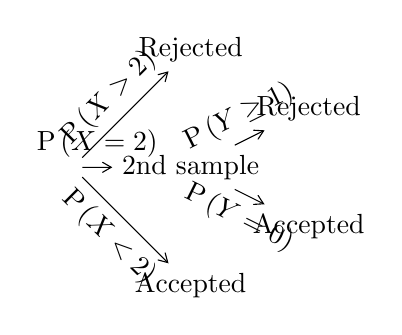
\begin{tikzpicture}[grow=right,->,>=angle 60,sloped] 
%\begin{scope}[yshift=0]
 \node {}
    child {node {Accepted}
            edge from parent
            node[below]  {$\text{P}\left(X<2\right)$}
    }
    child {node {2nd sample}
      child {node{Accepted}
       edge from parent
            node[below]  {$\text{P}\left(Y=0\right)$}
        }
      child {node {Rejected}
            edge from parent
            node[above]  {$\text{P}\left(Y\geq 1\right)$}
		}
        edge from parent
            node[above]  {$\text{P}\left(X=2\right)$}
    }
    child {node {Rejected}
        edge from parent
            node[above]  {$\text{P}\left(X>2\right)$}
}; 

%\end{scope}
\end{tikzpicture}
\end{center}

\begin{enumerate}[label=(\alph*)] 


\item  $X\sim\text{no. of pastries by junior chef that do not meet the passing standard, out of 12}$

$X\sim\text{B}\left(12,0.04\right)$

$
\begin{aligned}[t]
\text{P}\left(\text{accepted from the inspection of the 1st sample }\right) & =\text{P}\left(X<2\right)\\
 & =\text{P}\left(X\leq1\right)\\
 & =0.919\text{ (3 s.f.)}
\end{aligned}
$

\item  $Y\sim\text{no. of pastries by junior chef that do not meet the passing standard, out of 8}$

$Y\sim\text{B}\left(8,0.04\right)$

$
\begin{aligned}[t]
\text{P}\left(\text{rejected when a 2nd sample is selected for inspection}\right) & =\text{P}\left(X=2\right)\times\text{P}\left(Y\geq1\right)\\
 & =\text{P}\left(X=2\right)\times\left[1-\text{P}\left(Y=0\right)\right]\\
 & =0.0196\text{ (3 s.f.)}
\end{aligned}
$


\item 
$
\begin{aligned}[t]
\text{P}\left(\text{batch of pastries is rejected}\right) & =\text{P}\left(X>2\right)+\text{P}\left(X=2\right)\times\text{P}\left(Y\geq1\right)\\
 & =\left[1-\text{P}\left(X\leq2\right)\right]+\text{P}\left(X=2\right)\times\left[1-\text{P}\left(Y=0\right)\right]\\
 & =0.0303\text{ (3 s.f.)}
\end{aligned}
$

\item  The junior chef and the senior chef work independently. $2.5\%$
of the pastries made by the senior chef do not meet the passing standard.

\begin{enumerate}[label=(\roman*)] 

\item  $W\sim\text{no. of pastries by senior chef that do not meet passing standard, out of 6}$

$W\sim\text{B}\left(6,0.025\right)$

$
\begin{aligned}[t]
 & \text{P}\left(\text{exactly 2 pastries do not meet passing standard}\right)\\
 & =\text{P}\left(Y=2\right)\times\text{P}\left(W=0\right)+\text{P}\left(Y=0\right)\times\text{P}\left(W=2\right)+\text{P}\left(Y=1\right)\times\text{P}\left(W=1\right)\\
 & =0.0680\text{ (3 s.f.)}
\end{aligned}
$

\item  
$
\begin{aligned}[t]
\text{P}\left(\text{a pastry does not meet the passing standard}\right) & =0.4\left(0.04\right)+0.6\left(0.025\right)\\
 & =0.31
\end{aligned}
$

$A\sim\text{no. of pastries that do not meet the passing standard, out of 20}$

$A\sim\text{B}\left(20,0.031\right)$

$
\begin{aligned}[t]
\text{P}\left(\text{more than 3 do not meet the passing standard}\right) & =\text{P}\left(A>3\right)\\
 & =1-\text{P}\left(A\leq3\right)\\
 & =0.00300\text{ (3 s.f.)}
\end{aligned}
$

\end{enumerate}

\end{enumerate}

\end{example}

\chapter{Normal Distribution}
\section{The Normal Distribution}

The normal distribution is the \textbf{most important} distribution
for a continuous random variable. Many naturally occurring phenomena
have a distribution that is normal, or approximately normal. Some
examples are:

\begin{itemize}

\item  the height of an adult male, 

\item  the systolic blood pressure in healthy adults,

\item  the IQ scores of a large population.

\end{itemize}

\centerline{\begin{minipage}{.8\textwidth} 

While a discrete random variable is defined by its probability distribution,
a continuous random variable is defined by its \textbf{probability
density function}.

\begin{tcolorbox}[colback=blue!5, colframe=black, boxrule=.4pt, sharpish corners]

If $X$ is normally distributed then its probability density function
is given by 
\[
f\left(x\right)=\frac{1}{\sigma\sqrt{2\pi}}e^{-\frac{1}{2}\left(\frac{x-\mu}{\sigma}\right)^{2}}\quad\text{for}\:-\infty<x<\infty
\]
\end{tcolorbox}
\end{minipage}} 
\begin{center}
\includegraphics[width=14cm]{\string"../../../../Creative Cloud Files/NormalDistributionCurve\string".png}
\par\end{center}

If $X$ has a normal distribution with mean $\mu$ and variance $\sigma^{2}$
, we write
\[
X\sim\text{N}\left(\mu,\sigma^{2}\right)
\]

\centerline{\begin{minipage}{.8\textwidth} 
\begin{tcolorbox}[colback=blue!5, colframe=black, boxrule=.4pt, sharpish corners]

For a normal curve, the standard deviation is uniquely determined
as the horizontal distance from the line of symmetry $x=\mu$ to a
point of inflection.
\end{tcolorbox}
\end{minipage}} 

\newpage

\subsection{Properties of The Normal Distribution}

\begin{enumerate}

\item  The curve is bell shaped and \textbf{symmetrical about the
vertical line} $x=\mu$.

\item  The probability of any range of values is given by the \textbf{area
under the pdf} within that interval.

\item  The \textbf{total area} under the pdf curve is $\textbf{1}$.

\end{enumerate}
\begin{center}
\begin{tabular}{>{\centering}p{5cm}>{\centering}p{5cm}>{\centering}p{5cm}}
\centering{}\includegraphics[width=5cm]{\string"../../../../Creative Cloud Files/NormalDistributionCurve4\string".png} & \centering{}\includegraphics[width=5cm]{\string"../../../../Creative Cloud Files/NormalDistributionCurve5\string".png} & \centering{}\includegraphics[width=5cm]{\string"../../../../Creative Cloud Files/NormalDistributionCurve6\string".png}\tabularnewline
$\text{P}\left(X\leq a\right)$ & $\text{P}\left(X\geq a\right)$ & $\text{P}\left(a\leq X\leq b\right)$\tabularnewline
\end{tabular}
\par\end{center}

\begin{center}
\begin{tabular}{>{\centering}p{5cm}>{\centering}p{5cm}>{\centering}p{5cm}}
\centering{}\includegraphics[width=5cm]{\string"../../../../Creative Cloud Files/NormalDistributionCurve2\string".png} & \centering{}\includegraphics[width=5cm]{\string"../../../../Creative Cloud Files/NormalDistributionCurve3\string".png} & \centering{}\includegraphics[width=5cm]{\string"../../../../Creative Cloud Files/NormalDistributionCurve7\string".png}\tabularnewline
${\displaystyle \text{P}\left(X\leq\mu\right)=\frac{1}{2}}$ & ${\displaystyle \text{P}\left(X\geq\mu\right)=\frac{1}{2}}$ & $\text{Total Area}=1$\tabularnewline
\end{tabular}
\par\end{center}

Note: $\text{P}\left(X=a\right)=0$ since the corresponding area under
the curve is zero. Hence for a normal random variable, we have
\begin{align*}
\text{P}\left(X\leq a\right) & =\text{P}\left(X<a\right)+\text{P}\left(X=a\right)=\text{P}\left(X<a\right)\text{ and similarly,}\\
\text{P}\left(X\geq a\right) & =\text{P}\left(X>a\right)+\text{P}\left(X=a\right)=\text{P}\left(X\geq a\right)
\end{align*}


\subsection{Finding Probabilities Using Graphic Calculator}

For $X\sim\text{N}\left(\mu,\sigma^{2}\right)$, using the graphic
calculator: Press \tcbox[box align=base,nobeforeafter,colback=blue!40, colframe=blue!40,size=small]{\textbf{\textcolor{white}{2ND}}}\tcbox[box align=base,nobeforeafter,colback=black, colframe=black,size=small]{\textbf{\textcolor{white}{VARS}}}

\begin{itemize}

\item To find $\text{P}\left(X\leq b\right)$: Select 2:normalcdf
and key the values in the format $10^{-99}$, $b$, $\mu$, $\sigma$.

\item  To find $\text{P}\left(X\geq a\right)$: Select 2:normalcdf
and key the values in the format $a$, $10^{99}$, $\mu$, $\sigma$.

\item  To find $\text{P}\left(a\leq X\leq b\right)$: Select 2:normalcdf
and key the values in the format $a$, $b$, $\mu$, $\sigma$.

\item  To find $a$ such that $\text{P}\left(X\leq a\right)=p$ :
Select 3:invNorm and key the values in the format $p$, $\mu$, $\sigma$,
tail.

\end{itemize}

Note: Remember to enter $\sigma$ (standard deviation) and not $\sigma^{2}$
(variance) when using the GC.

\begin{example}[Finding Probabilities of Normal Distributions (Area Under The Curve)]

The weight of a randomly chosen student from a population may be assumed
to have a normal distribution with mean $65\,\text{kg}$ and standard
deviation $3\,\text{kg}$. A student was randomly chosen from this
population. Find the proabability that

\begin{enumerate}[label=(\alph*)] 

\item  his weight exceeds $\text{70}\,\text{kg}$,

\item  his weight is below $\text{62}\,\text{kg}$,

\item  his weight is between $60\,\text{kg}$ and $75\,\text{kg}$,

\item  his weight is within one standard deviation from the mean
weight.

\end{enumerate}

\Solution

Let $X$ be the weight of a randomly chosen student

$X\sim\text{N}\left(65,9\right)$

\begin{enumerate}[label=(\alph*)] 

\item  $\text{P}\left(X>70\right)=0.478\text{ (3 s.f.)}$

\item  $\text{P}\left(X<62\right)=0.159\text{ (3 s.f.)}$

\item  $\text{P}\left(60<X<75\right)=0.952\text{ (3 s.f.)}$

\item  
$
\begin{aligned}[t]
\text{P}\left(\left|X-65\right|<3\right) & =\text{P}\left(62<X<68\right)\\
 & =0.683\text{ (3 s.f.)}
\end{aligned}
$

\end{enumerate}

\end{example}

\begin{example}[Inverse Normal Values]

Given $X\sim\text{N}\left(10,4\right)$, find, correct to 3 significant
figures, the values of $a$, $b$ and $c$ such that

\begin{enumerate}[label=(\alph*)] 

\item  $\text{P}\left(X\leq a\right)=0.15$

\item  $\text{P}\left(X\geq b\right)=0.23$

\item  $\text{P}\left(9<X<c\right)=0.64$

\end{enumerate}

\Solution

\begin{enumerate}[label=(\alph*)] 

\item  

\begin{minipage}[t]{.6\textwidth}

From GC, $a=7.93\text{ (3 s.f.)}$

\includegraphics[width=4cm]{\string"../../JC Statistics/GC Screenshots/invNorm1\string".png}\hspace{1cm}\includegraphics[width=4cm]{\string"../../JC Statistics/GC Screenshots/invNorm2\string".png}

\end{minipage}
\begin{minipage}[t]{.3\textwidth}
\begin{center}
\includegraphics[width=5cm,valign=t]{\string"../../../../Creative Cloud Files/NormalExInvNorm1\string".png}
\par\end{center}

\end{minipage}

\item  \begin{minipage}[t]{.6\textwidth}

From GC, $b=11.5\text{ (3 s.f.)}$

\includegraphics[width=4cm]{\string"../../JC Statistics/GC Screenshots/invNorm3\string".png}\hspace{1cm}\includegraphics[width=4cm]{\string"../../JC Statistics/GC Screenshots/invNorm4\string".png}

\end{minipage}
\begin{minipage}[t]{.3\textwidth}
\begin{center}
\includegraphics[width=5cm,valign=t]{\string"../../../../Creative Cloud Files/NormalExInvNorm2\string".png}
\par\end{center}

\end{minipage}

\item 
$
\begin{aligned}[t]
\text{P}\left(X<c\right)-\text{P}\left(X<9\right) & =0.64\\
\text{P}\left(X<c\right) & =0.64+\text{P}\left(X<9\right)\\
 & =0.94854\text{ (5 s.f.)}
\end{aligned}
$

\begin{minipage}[t]{.6\textwidth}

From GC, $c=13.3\text{ (3 s.f.)}$

\includegraphics[width=4cm]{\string"../../JC Statistics/GC Screenshots/invNorm5\string".png}\hspace{1cm}\includegraphics[width=4cm]{\string"../../JC Statistics/GC Screenshots/invNorm6\string".png}

\end{minipage}
\begin{minipage}[t]{.3\textwidth}
\begin{center}
\includegraphics[width=5cm,valign=t]{\string"../../../../Creative Cloud Files/NormalExInvNorm3\string".png}
\par\end{center}

\end{minipage}

\end{enumerate}

\end{example}

\section{The Standard Normal Distribution (Z-Distribution)}

The standard normal distribution with mean $\mu=0$ and standard deviation $\sigma=1$ is denoted by $Z$, i.e. 

$Z\sim\text{N}\left(0,1\right)$. 

Every normal distribution can be transformed into the standard normal
distribution or $Z-$distribution using the transformation ${\displaystyle Z=\frac{X-\mu}{\sigma}}$. 

This process of converting $X\sim\text{N}\left(\mu,\sigma^{2}\right)$
into $Z\sim\text{N}\left(0,1\right)$ is known as standardisation.

We usually perform standardisation when $\mu$ and/or $\sigma$ are
unknown.

\begin{example}[Standardisation to Find $\mu$]

Given that $X\sim\text{N}\left(\mu,0.04\right)$ and $\text{P}\left(X<5\right)=0.3$,
find $\mu$.

\Solution

\begin{align*}
\text{P}\left(X<5\right) & =0.3\\
\text{P}\left(Z<\frac{5-\mu}{\sqrt{0.04}}\right) & =0.3
\end{align*}

From GC,
\begin{align*}
\frac{5-\mu}{0.2} & =-0.52440\text{ (5 s.f.)}\\
\mu & =5.10\text{ (3 s.f.)}
\end{align*}

\end{example}

\begin{example}[Standardisation to Find $\sigma$]

Given that $X\sim\text{N}\left(12,\sigma^{2}\right)$ and $\text{P}\left(X\geq15\right)=0.0668$,
find the standard deviation of $X$.

\Solution

\begin{align*}
\text{P}\left(X\geq15\right) & =0.0668\\
\text{P}\left(Z<\frac{15-12}{\sigma}\right) & =0.0668
\end{align*}

From GC, 
\begin{align*}
\frac{3}{\sigma} & =1.5001\text{ (5 s.f.)}\\
\sigma & =2.00\text{ (3 s.f.)}
\end{align*}

\end{example}

\newpage

\begin{example}[Standardisation to Find $\mu$ and $\sigma$]

In a particular town, $34$ out of $100$ people have heights exceeding
$1.65\,\text{m}$ and $4$ out of $5$ people have heights below $1.8\,\text{m}$.
Assuming that their heights follow a normal distribution, find the
mean and standard deviation of the distribution. 

\Solution

Let $X$ be the height of a randomly chosen person from the town.

$X\sim\text{N}\left(\mu,\sigma^{2}\right)$

Given that $\text{P}\left(X>1.65\right)=0.34$, 

\begin{align*}
\text{P}\left(X>1.65\right) & =0.34\\
\text{P}\left(Z>\frac{1.65-\mu}{\sigma}\right) & =0.34\\
\text{P}\left(Z\leq\frac{1.65-\mu}{\sigma}\right) & =0.66\\
\frac{1.65-\mu}{\sigma} & =0.41246\text{ (5 s.f.)}
\end{align*}

and given that $\text{P}\left(X<1.8\right)=0.8$, 
\begin{align*}
\text{P}\left(X<1.8\right) & =0.8\\
\text{P}\left(Z\leq\frac{1.8-\mu}{\sigma}\right) & =0.8\\
\frac{1.8-\mu}{\sigma} & =0.84162\text{ (5 s.f.)}
\end{align*}

Rearranging the equations, we have the following simultaneous equations:

\begin{align*}
\mu+0.41246\sigma & =1.65\cdots\cdots(1)\\
\mu+0.84162 & =1.8\cdots\cdots(2)
\end{align*}

Using GC to solve (1) and (2), $\mu=1.51$ and $\sigma=0.350$.

\end{example}

\newpage

\section{Linear Combinations of Normal Random Variables}

Recall that we have the following properties for the expectation and
variance of two random variables.

\medskip

\centerline{\begin{minipage}{\textwidth} 
\begin{tcolorbox}[colback=blue!5, colframe=black, boxrule=.4pt, sharpish corners]

For any random variables $X$ and $Y$, and constants $a$ and $b$,

\medskip{}

\begin{minipage}[t]{0.5\textwidth} 

\begin{enumerate}[label=(\alph*)] 

\item  $\text{E}\left(a\right)=a$

\item  $\text{E}\left(aX\right)=a\text{E}\left(X\right)$

\item  $\text{E}\left(aX\pm b\right)=a\text{E}\left(X\right)\pm b$

\item  $\text{E}\left(aX\pm bY\right)=a\text{E}\left(X\right)\pm b\text{E}\left(Y\right)$

\end{enumerate}

\end{minipage}
\begin{minipage}[t]{0.5\textwidth} 

\begin{enumerate}[label=(\alph*)] 

\item  $\text{Var}\left(a\right)=0$

\item $\text{Var}\left(aX\right)=a^{2}\text{Var}\left(X\right)$

\item $\text{Var}\left(aX\pm b\right)=a^{2}\text{Var}\left(X\right)$

\item  If $X$ and $Y$ are \textbf{independent}, then

$\text{Var}\left(aX\pm bY\right)=a^{2}\text{Var}\left(X\right)+b^{2}\text{Var}\left(Y\right)$

\end{enumerate}

\end{minipage}
\end{tcolorbox}
\end{minipage}}

\medskip


If $X$ and $Y$ are two \textbf{independent normal} random variables,
and $a$ and $b$ are non zero constants, then

\[
aX\pm bY\:\text{are also normal random variables.}
\]

Thus, if $X\sim\text{N}\left(\mu_{1},\sigma_{1}^{2}\right)$ and $Y\sim\text{N}\left(\mu_{2},\sigma_{2}^{2}\right)$
are independent random variables, and $a$ and $b$ are non zero constants,
then

\begin{enumerate}[label=(\alph*)]

\item $aX\sim\text{N}\left(a\mu_{1},a^{2}\sigma_{1}^{2}\right)$

\item $aX\pm b\sim\text{N}\left(a\mu_{1}\pm b,a^{2}\sigma_{1}^{2}\right)$

\item $aX\pm bY\sim\text{N}\left(a\mu_{1}\pm b\mu_{2},a^{2}\sigma_{1}^{2}+b^{2}\sigma_{2}^{2}\right)$

\end{enumerate}

\begin{example}[Finding Distribution of Linear Combinations of Normal Random Variables]

Given $X$ and $Y$ are independent with $X\sim\text{N}\left(3,9\right)$
and $Y\sim\text{N}\left(1,4\right)$

State the distribution of:

\begin{tasks}[label=(\alph*),label-width=3.5ex](2) 

\task  $2X$

\task  $X+3$

\task  $X+2Y$

\task  $X-2Y$

\task  $X_{1}+X_{2}+X_{3}+Y_{1}+Y_{2}$, where $X_{1},X_{2},X_{3}$
are independent observations of $X$ and $Y_{1},Y_{2}$ independent
observations of $Y$.

\end{tasks}

\Solution

\begin{tasks}[label=(\alph*),label-width=3.5ex](2) 

\task  $2X\sim\text{N}\left(6,36\right)$

\task  $X+3\sim\text{N}\left(6,9\right)$

\task  $X+2Y\sim\text{N}\left(5,25\right)$

\task  $X-2Y\sim\text{N}\left(1,25\right)$

\task  $X_{1}+X_{2}+X_{3}+Y_{1}+Y_{2}\sim\text{N}\left(11,35\right)$

\end{tasks}

\end{example}

\newpage

\begin{example}[Heights of Males vs Females]

In a particular town, the heights, in centimetres, of the males and
females are normally distributed as follows:
\begin{center}
\setlength{\extrarowheight}{2pt}%
\begin{tabular}{|>{\centering}p{4cm}|>{\centering}p{4cm}|>{\centering}p{4cm}|}
\hline 
 & Mean & Variance\tabularnewline
\hline 
Male & $177$ & $18.4$\tabularnewline
\hline 
Female & $162$ & $13.2$\tabularnewline
\hline 
\end{tabular}
\par\end{center}

\begin{enumerate}[label=(\alph*)] 

\item  Find the probability that a randomly chosen female is taller
than a randomly chosen male.

\item  Find the probability that the total height of three randomly
chosen females exceeds that of $2$ randomly chosen males by more
than $100\,\text{cm}$.

\end{enumerate}

\Solution

Let $X$ be the height of a randomly chosen male from the town.

$X\sim\text{N}\left(177,18.4^{2}\right)$

Let $Y$ be the height of a randomly chosen female from the town.

$Y\sim\text{N}\left(162,13.2^{2}\right)$

\begin{enumerate}[label=(\alph*)] 

\item  $Y-X\sim\text{N}\left(-15,512.8\right)$

\begin{align*}
\text{P}\left(Y>X\right) & =\text{P}\left(Y-X>0\right)\\
 & =0.254\text{ (3 s.f.)}
\end{align*}

\item  $\left(Y_{1}+Y_{2}+Y_{3}\right)-\left(X_{1}+X_{2}\right)\sim\text{N}\left(132,1199.84\right)$

\[
\text{P}\left(Y_{1}+Y_{2}+Y_{3}-X_{1}+X_{2}>100\right)=0.822\text{ (3 s.f.)}
\]

\end{enumerate}

\end{example}

\begin{example}[Mass of Papayas]

Papayas are sold by mass. The masses, in kg, of papayas follow a normal distribution with mean $0.7$ and standard deviation $6.1$.

Find the probability that the total mass of $2$ randomly chosen papayas
is heavier than twice the mass of a randomly chosen papaya by at most
$80\,\text{g}$.

\Solution

Let $X$ be the mass of a randomly chosen papaya

$X\sim\text{N}\left(0.7,6.1^{2}\right)$

$\left(X_{1}+X_{2}\right)-2X\sim\text{N}\left(0,223.26\right)$

\[
\text{P}\left(X_{1}+X_{2}-2X<0.08\right)=0.502\text{ (3 s.f.)}
\]

\end{example}

\newpage{}



\chapter{Sampling Distribution (Central Limit Theorem)}

\section{Population and Sample}

When we need to gather information about a \textbf{population}, very
rarely in practice can we afford the luxury of examining the complete
population. The two obvious reasons would be that the cost is too
high and the population is dynamic in that the individuals making
up the population may change over time.

Commonly, \textbf{sample} observations and analyses are used to make inferences or predictions about a population. That is, we take the
results of an analysis using a sample and generalize it to the larger
population that the sample represents. This is known as \textit{statistical inference}.

\medskip

\centerline{\begin{minipage}{.68\textwidth} 
\begin{tcolorbox}[colback=blue!5, colframe=black, boxrule=.4pt, sharpish corners]

A \textbf{population} is the whole set of items that we want to study.

A \textbf{sample} is a subset of the population.
\end{tcolorbox}
\end{minipage}} 

\medskip


In order for the statistical inference to be as accurate as possible,
however, it is imperative that the sample is representative of the
population (i.e. accurately reflect the characteristics of the population)
to which it is being generalized. As such, the sample must be carefully
gathered through \textbf{random sampling}.

\section{Random Sampling}

\centerline{\begin{minipage}{.68\textwidth} 
\begin{tcolorbox}[colback=blue!5, colframe=black, boxrule=.4pt, sharpish corners]

In \textbf{random sampling}, every element in the population must
have an equal chance of selection, i.e. it is free from bias.
\end{tcolorbox}
\end{minipage}} 

\medskip

In non-random sampling, each element in the population does not have
an equal chance of being selected, resulting in certain segments of
the population being over represented, as some members are systematically or deliberately excluded from study.

\begin{example}[Random Sampling Methods]

In a small school there are 3 classes, each with 30 students, and
2 classes, each with 20 students. To find the students perception
of the food sold in a canteen, a sample of 10 students is taken by
the following three methods. 

\begin{enumerate}[label=Method \arabic*:, leftmargin=2cm]

\item  2 students are randomly chosen from each of the 5 classes.

\item  Assign every student in the school with a number from 1 to
130 by arranging their names in alphabetical order. Use a computer
to generate 10 random numbers. The 10 students with the corresponding
numbers would be the ones chosen to be in the sample.

\item  The first 10 students who patrionize the chicken rice stall
are selected as the sample.

\end{enumerate}

\Solution

In choosing a random sample, each member of the population must have an equal chance of being selected.

\uline{Method 1}

Let $A$ be the event that a particular student from the class of
$20$ is chosen.

\begin{align*}
\text{P}\left(A\right) & =\frac{1}{10}
\end{align*}

Let $B$ be the event that a particular student from the class of
$30$ is chosen.
\begin{align*}
\text{P}\left(B\right) & =\frac{1}{15}
\end{align*}
Since the probability of choosing any one student is not equal, this
method does not involve random sampling.

\uline{Method 2}

Since each student has a probability of ${\displaystyle \frac{1}{13}}$
of being chosen, this method does involve random sampling.

\uline{Method 3}

This method does not involve random sampling because students who
do not eat chicken rice will not patrionize the chicken rice stall
and thus will not be selected.

\end{example}

\section{Population Parameters and Sample Statistics}

\centerline{\begin{minipage}{.65\textwidth} 
\begin{tcolorbox}[colback=blue!5, colframe=black, boxrule=.4pt, sharpish corners]

A \textbf{population parameter} is a number that is characteristic
of the population under study.
\end{tcolorbox}
\end{minipage}} 

\medskip

A population parameter is a number that is characteristic of the population under study.

In many cases, we are concerned with two population parameters, 

\begin{itemize}

\item  \textbf{population mean }

\item  \textbf{population variance}

\end{itemize}

These are constants of a population and they are often unknown. The
study of a population often involves finding estimates of these parameters.

\medskip

\centerline{\begin{minipage}{.6\textwidth} 
\begin{tcolorbox}[colback=blue!5, colframe=black, boxrule=.4pt, sharpish corners]

A \textbf{sample statistic} is a number that is characteristic of
a sample drawn from the population.
\end{tcolorbox}
\end{minipage}} 

\medskip

In general, a sample statistic is a \textbf{random variable} which
contains information about the sample while any corresponding population parameter is a (possibly unknown) constant.

We use the following notation for parameters and statistics.\setlength{\extrarowheight}{2pt}

\begin{tabular}{|>{\centering}m{3.5cm}|>{\centering}m{3.5cm}|>{\centering}m{3.5cm}|>{\centering}m{3.5cm}|}
\hline 
\multirow{2}{3.5cm}{\hspace{31bp}Quantity} & \multirow{2}{3.5cm}{\hspace{25bp}Population} & \multicolumn{2}{c|}{Sample}\tabularnewline
\cline{3-4} \cline{4-4} 
 &  & As a random variable & As a possible value\tabularnewline
\hline 
Mean & $\mu$ & $\overline{X}$ & $\overline{x}$\tabularnewline
\hline 
Variance & $\sigma^{2}$ & $\sigma_{X}^{2}$ & $\sigma_{x}^{2}$\tabularnewline
\hline 
\end{tabular}

\newpage


\section{The Sample Mean, $\textbf{\ensuremath{\overline{X}}}$ as a Random Variable}

Let $X_{1},X_{2},X_{3},...,X_{n}$ be $n$ independent observations
taken from a population $X$, with mean $\mu$ and variance $\sigma^{2}$.

Then the sample mean $\overline{X}$, defined by 
\[
\overline{X}=\frac{X_{1}+X_{2}+X_{3}+\ldots+X_{n}}{n}
\]
is a random variable with $\text{E}\left(\overline{X}\right)=\mu$
and ${\displaystyle \text{Var}\left(\overline{X}\right)=\frac{\sigma^{2}}{n}}$.

\begin{fleqn}

\textbf{Proof}:

\begin{minipage}[t]{0.5\textwidth} 

\begin{align*}
\text{E}\left(\overline{X}\right) & =\text{E}\left(\frac{X_{1}+X_{2}+X_{3}+\ldots+X_{n}}{n}\right)\\
 & =\frac{1}{n}\text{E}\left(X_{1}+X_{2}+X_{3}+\ldots+X_{n}\right)\\
 & =\frac{1}{n}\left(n\text{E}\left(X\right)\right)\\
 & =\mu
\end{align*}

\end{minipage}
\hfill\vline\hfill 
\begin{minipage}[t]{0.5\textwidth} 

$
\begin{aligned}[t]
\text{Var}\left(\overline{X}\right) & =\text{Var}\left(\frac{X_{1}+X_{2}+X_{3}+\ldots+X_{n}}{n}\right)\\
 & =\frac{1}{n^{2}}\text{Var}\left(X_{1}+X_{2}+X_{3}+\ldots+X_{n}\right)\\
 & =\frac{1}{n^{2}}\left(n\text{Var}\left(X\right)\right)\\
 & =\frac{\sigma^{2}}{n}
\end{aligned}
$

\end{minipage}

\end{fleqn}

\section{Distribution of $\textbf{\ensuremath{\overline{X}}}$ }

\subsection{When $X$ Follows a Normal Distribution}

\begin{tcolorbox}[colback=blue!5, colframe=black, boxrule=.4pt, sharpish corners]

If $X_{1},X_{2},X_{3},...,X_{n}$ are $n$ independent observations
from a \textbf{normal distribution} with mean $\mu$ and variance
$\sigma^{2}$, then the sample mean $\overline{X}$ is also normally
distributed such that 
\[
\overline{X}\sim\text{N}\left(\mu,\frac{\sigma^{2}}{n}\right)\:\textbf{exactly}
\]

\end{tcolorbox}

\begin{example}[Sample Mean of a Normal Distribution]

A random sample of size $15$ is taken from a population which is
normally distributed with mean $60$ and standard deviation $4$.
Find the probability that the mean of the sample is less than $58$.

\Solution

Let ${\displaystyle X\sim\text{N}\left(60,4^{2}\right)}$

${\displaystyle \overline{X}\sim\text{N}\left(60,\frac{4^{2}}{15}\right)}\:\text{exactly}$

Using GC, 
\[
\text{P}\left(\overline{X}<58\right)=0.0264
\]
\end{example}

\newpage

\begin{example}[Finding $n$ By Standardization]

A large number of random samples of size $n$ are taken from a normal
population with mean 74 and variance 36 and the sample means are calculated.
If at most $85\%$ of the sample means exceed $72$, find the largest
possible value of $n$.

\Solution

Let ${\displaystyle X\sim\text{N}\left(74,36\right)}$

${\displaystyle \overline{X}\sim\text{N}\left(74,\frac{36}{n}\right)}\:\text{exactly}$

Given $\text{P}\left(\overline{X}>72\right)\leq0.85$,

\begin{align*}
\text{P}\left(Z>\frac{72-74}{\sqrt{\frac{36}{n}}}\right) & \leq0.85\\
\text{P}\left(Z>-\frac{\sqrt{n}}{3}\right) & \leq0.85\\
-\frac{\sqrt{n}}{3} & \leq-1.0364(\text{5 s.f.})\\
n & \leq9.67(\text{3 s.f.})
\end{align*}
Thus the largest possible value of $n$ is $9$.

\end{example}

\subsection{When $X$ Follows Any Distribution (Central Limit Theorem)}

\begin{tcolorbox}[colback=blue!5, colframe=black, boxrule=.4pt, sharpish corners]

If $X_{1},X_{2},X_{3},...,X_{n}$ are $n$ independent observations
from \textbf{ANY distribution}, $\boldsymbol{X}$, with mean $\mu$ and variance
$\sigma^{2}$, then when $n$ is sufficiently large $\left(n\geq30\right)$,
by the \textbf{Central Limit Theorem}, 
\[
\overline{X}\sim\text{N}\left(\mu,\frac{\sigma^{2}}{n}\right)\:\textbf{approximately}
\]

\end{tcolorbox}

\begin{example}[Sample Mean of a Binomial Distribution Using CLT]

Ten fair die are thrown and the number of sixes is recorded. If the
experiment is repeated $50$ times and the number of sixes are recorded
each time, estimate the probability that the mean number of sixes
in each experiment will be less than $1.6$. 

\Solution
Let $X$ be the no. of sixes out of 10 fair die.

${\displaystyle X\sim\text{B}\left(10,\frac{1}{6}\right)}$

\begin{align*}
\text{E}\left(X\right) & =np=\frac{5}{3}\qquad\qquad\text{Var}\left(X\right)=np\left(1-p\right)=\frac{25}{18}
\end{align*}

Since the sample size $n=50$ is sufficiently large $\left(\geq30\right)$,
by the Central Limit Theorem,
\[
\overline{X}\sim\text{N}\left(\frac{5}{3},\frac{1}{36}\right)\:\text{approximately}
\]

Thus,
\[
\text{P}\left(\overline{X}<1.6\right)=0.345(\text{3 s.f.})
\]
\end{example}

\begin{example}[Sample Mean of a Probability Distribution Using CLT]

A random variable $X$ has the probability distribution shown in the
table below. The sample mean for 50 independent observations of $X$
is denoted by $\overline{X}$. Using a suitable approximation, find
$\text{P}\left(\overline{X}>0\right)$.
\begin{center}
\begin{tabular}{|>{\centering}m{2cm}|>{\centering}m{2cm}|>{\centering}m{2cm}|>{\centering}m{2cm}|>{\centering}m{2cm}|>{\centering}m{2cm}|}
\hline 
$x$ & $-2$ & $-1$ & $0$ & $1$ & $2$\tabularnewline
\hline 
$\text{P}\left(X=x\right)$ & $0.3$ & $0.1$ & $0.15$ & $0.4$ & $0.05$\tabularnewline
\hline 
\end{tabular}
\par\end{center}

\Solution

\begin{align*}
\text{E}\left(X\right) & =-2\left(0.3\right)-1\left(0.1\right)+0+1\left(0.4\right)+2\left(0.05\right)\\
 & =-0.2
\end{align*}
\begin{align*}
\text{E}\left(X^{2}\right) & =4\left(0.3\right)+1\left(0.1\right)+0+1\left(0.4\right)+4\left(0.05\right)\\
 & =1.9
\end{align*}

\begin{align*}
\text{Var}\left(X\right) & =\text{E}\left(X^{2}\right)-\left[\text{E}\left(X\right)\right]^{2}\\
 & =1.86
\end{align*}
Since the sample size $n=50$ is sufficiently large $\left(\geq30\right)$,
by the Central Limit Theorem,
\[
\overline{X}\sim\text{N}\left(-0.2,\frac{1.86}{50}\right)\:\text{approximately}
\]
\[
\text{P}\left(\overline{X}>0\right)=0.150(\text{3 s.f.})
\]

\end{example}


\section*{Central Limit Theorem Summary}


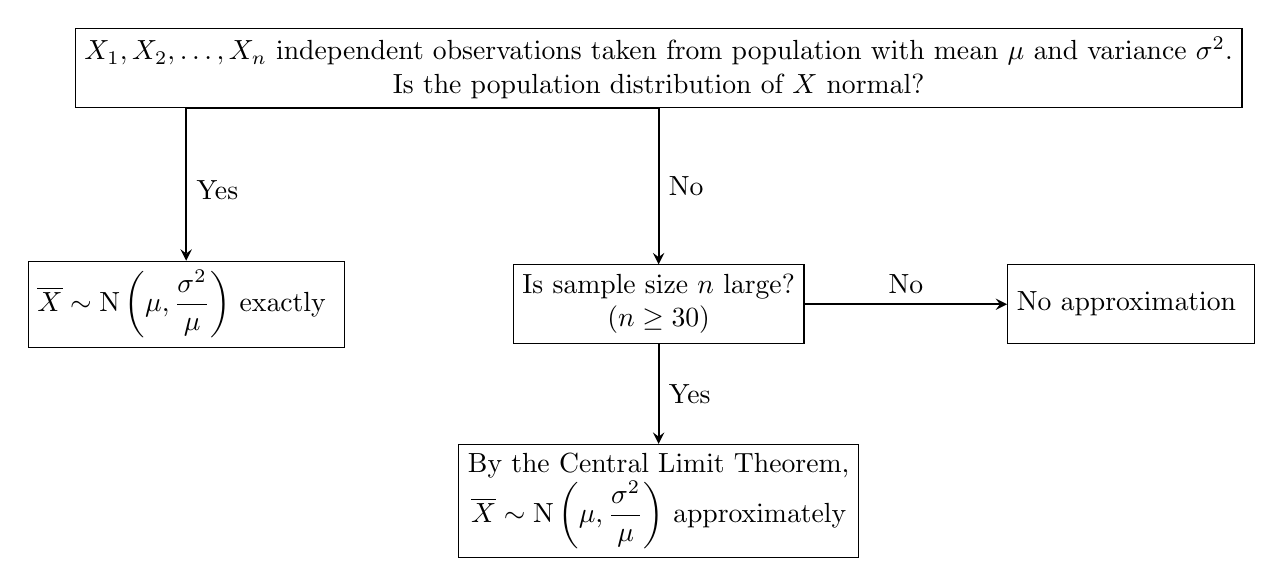
\begin{tikzpicture}[every text node part/.style={align=center}]
\node (Population Distribution)[Box]{$X_{1},X_{2},\ldots,X_{n}$ independent observations taken from population with mean $\mu$ and variance $\sigma^{2}$.\\

Is the population distribution of $X$ normal?
};
\node (Not Exact)[Box, below of = Population Distribution, yshift=-2cm]{Is sample size $n$ large? \\
$\left(n\geq30\right)$
};

\node (Exact)[Box, left of = Not Exact,xshift=-5cm]{${\displaystyle \overline{X}\sim\text{N}\left(\mu,\frac{\sigma^{2}}{\mu}\right)}$
exactly
};

\node (Not large)[Box, right of = Not Exact,xshift=5cm]{ No approximation
};

\node (CLT)[Box, below of = Not Exact,yshift=-1.5cm]{ By the Central Limit Theorem,  \\

$
{\displaystyle \overline{X}\sim\text{N}\left(\mu,\frac{\sigma^{2}}{\mu}\right)}\text{ approximately}
$
};


\draw[arrow](Population Distribution)--(Not Exact)node[midway, right]{No};
\draw[arrow](Population Distribution.south)-|(Exact.north)node[right,yshift=.9cm]{Yes};
\draw[arrow](Not Exact.east)--(Not large.west)node[midway,above]{No};
\draw[arrow](Not Exact.south)--(CLT.north)node[midway,right]{Yes};



\end{tikzpicture}


\chapter{Hypothesis Testing}
A manufacturer claims that the light bulbs he produces have a mean
lifespan of $600$ hours, and a standard deviation of $60$ hours.
In statistics, we call this a \textbf{statistical hypothesis}. 

A retailer, having received numerous complaints from his customers,
suspects that they do not last as long. He contacts the manufacturer
and they decide to test a random sample of $50$ bulbs. It turns out
that the average lifespan of this sample, $\overline{x}$, is $580$
hours.

\begin{minipage}[t]{.65\textwidth}

Is this proof that the average lifespan of their light bulbs is below
$600$ hours? It is possible that the average lifespan of the population
is actually $600$ and that the sampled light bulbs just had a lower
than average lifespan. Our sample cannot tell us with certainty the
exact population mean $\mu$. How do we then decide between the validity
of manufacturer's claim and that of the angry customers?

\medskip

Statisticians have devised a procedure to determine whether a statistical
hypothesis is reasonable. We call it a \textbf{hypothesis test}.

\end{minipage}
\begin{minipage}[t]{.35\textwidth}
\begin{center}
\includegraphics[width=5cm,valign=t]{\string"../../../../Creative Cloud Files/ManLooksAtLightBulb\string".png}
\par\end{center}

\end{minipage}

\medskip

\centerline{\begin{minipage}{.7\textwidth} 
\begin{tcolorbox}[colback=blue!5, colframe=black, boxrule=.4pt, sharpish corners]

A \textbf{statistical hypothesis} is an assertion or conjecture\footnotemark
concerning one or more populations.
\end{tcolorbox}
\end{minipage}} 

\footnotetext{An opinion or conclusion formed on the basis of incomplete information.} 

\medskip

To prove that a hypothesis is true, or false, with absolute certainty,
we would need absolute knowledge. That is, we would have to examine
the entire population. In most cases, it would be very silly to examine
the entire population. For example if the light bulb manufacturer
were to test the lifespan every light bulb he produces, he would have
no light bulbs left to sell. Instead, hypothesis testing concerns
on how to use a random sample to judge if it is evidence that supports
or not the hypothesis.

\section{Null and Alternative Hypotheses}

Suppose a claim is made that a population mean $\mu$ has a value
$\mu_{0}$. We call this the \textbf{null hypothesis} $H_{0}$, and
we write 
\[
H_{0}:\mu=\mu_{0}
\]

This statement is assumed to be true unless we have enough evidence
to reject it.

The alternative hypothesis, denoted by $H_{1}$, is used to contradict
the null hypothesis. 

If $H_{0}$ is not rejected, we accept that the population mean in
$\mu_{0}$.

If $H_{0}$ is rejected, we accept that there is a difference between
$\mu$ and $\mu_{0}$. 

\medskip

\begin{tcolorbox}[colback=blue!5, colframe=black, boxrule=.4pt, sharpish corners]

Given the null hypothesis $H_{0}:\mu=\mu_{0}$, there are three ways to set up the alternative hypothesis:

\begin{itemize}
  \item $H_{1}:\mu>\mu_{0}$

  \item $H_{1}:\mu<\mu_{0}$
	\makebox(0,0){\put(0,3\normalbaselineskip){%
            $\left.\rule{0pt}{1.4\normalbaselineskip}\right\}$ \textbf{One-tail Test}}}
  \item $H_{1}:\mu\neq\mu_{0}$ \hspace{.33cm} \textbf{Two-tail Test}

\end{itemize} 
\end{tcolorbox}

\medskip

Consider the light bulb example given at the start. The manufacturer
claims (null hypothesis) that his light bulbs have a lifespan of $600$
hours. We write, $H_{0}:\mu=600$. 

The retailer's suspicion that this claim is over-estimated (alternative
hypothesis) is written formally as $H_{1}:\mu<600$.

\begin{example}[Null and Alternative Hypothesis]

For each of the following scenarios, write down the null and alternative
hypotheses. State whether a one-tail or two tail test applies.

\begin{enumerate}[label=(\alph*)]

\item  The top speed of submarines currently being produced by a
manufacturer is currently $26.3$ knots. When their engineers modify
the design to reduce drag, they believe the maximum speed will be
increased.

\item  The average peak-hour travel time along a particular stretch
of road is currently $27$ minutes. To help reduce travel times, electronic
signs displaying real-time information are erected. If the travel
times improve, the signs will be widely implemented. 

\item  Whitex produces copy paper, and the weight of the copy paper
is given as $80\,\text{g per m}^{2}$. The company wants to determine
whether this information is correct.

\end{enumerate}

\Solution

\begin{tasks}[label=(\alph*),label-width=3.5ex](3)

\task  $H_{0}:\mu=26.3$, $H_{1}:\mu>26.3$

One-tail test

\task  $H_{0}:\mu=27$, $H_{1}:\mu<27$

One-tail test

\task  $H_{0}:\mu=80$, $H_{1}:\mu\neq80$

Two-tail test

\end{tasks}

\end{example}

\section{Hypothesis Testing}

\subsection{The Test Statistic}

To carry out the test, our focus moves from $X$ (e.g. the lifespan
of light bulbs) to the distribution of $\overline{X}$ (e.g. the mean
lifespan from a sample of lightbulbs). $\overline{X}$ is called the
\textbf{test statistic} for the population mean $\mu$. The decision
to reject or not to reject $H_{0}$ depends on how far the observed
sample mean, $\overline{x}$, is from the claimed mean. 

\begin{tcolorbox}[colback=blue!5, colframe=black, boxrule=.4pt, sharpish corners]

A \textbf{test statistic} is a random variable that is calculated
from sample data (e.g. sample mean).

\medskip

The distribution of the test statistic under the assumptions of $H_{0}$
is called the \textbf{null distirbution}.
\end{tcolorbox}

We have seen that for a population which is normally distributed with
mean $\mu$ and standard deviation $\sigma$, the sample mean 

\[
\overline{X}\sim\text{N}\left(\mu,\frac{\sigma^{2}}{n}\right)\text{ exactly}
\]

If the population is not normally distributed but the sample size
is sufficiently large, we can apply the Central Limit Theorem 

\[
\overline{X}\sim\text{N}\left(\mu,\frac{\sigma^{2}}{n}\right)\text{ approximately}
\]

Under the assumptions of $H_{0}$, $\mu=\mu_{0}$, so our null distribution
is ${\displaystyle \overline{X}\sim\text{N}\left(\mu_{0},\frac{\sigma^{2}}{n}\right)}$. 

In our light bulb example, $H_{0}:\mu=600$. Under the assumption
that the null hypothesis is true, the population mean and standard
deviation are $\mu=600$ and $\sigma=60$ (these are the values given
by the manufacturer). Our sample size $n$ is $50$. So, by the Central
Limit Theorem, we have the null distribution

\[
\overline{X}\sim\text{N}\left(600,\frac{60^{2}}{50}\right)\text{ approximately, since \ensuremath{n=50} is sufficiently large}
\]

However in hypothesis testing, we will not be using the test statistic
$\overline{X}$. Instead, the standardised test statistic is used, 

\[
Z=\frac{\overline{X}-\mu_{0}}{\frac{\sigma}{\sqrt{n}}},\text{ where }Z\sim\text{N}\left(0,1\right)
\]

\begin{tcolorbox}[colback=blue!5, colframe=black, boxrule=.4pt, sharpish corners]

Consider a statistical hypothesis test of $H_{0}:\mu=\mu_{0}$ for
a normally distributed population with known standard deviation $\sigma$.
Given a sample of size $n$ with observed sample mean $\overline{x}$:

The standardised test statistic is ${\displaystyle Z=\frac{\overline{X}-\mu_{0}}{\frac{\sigma}{\sqrt{n}}}},\text{ where }Z\sim\text{N}\left(0,1\right)$ 

which has observed value ${\displaystyle z=\frac{\overline{x}-\mu_{0}}{\frac{\sigma}{\sqrt{n}}}}$.
\end{tcolorbox}

Back to the light bulb example:

The population standard deviation is $60$ hours.

When they take a random sample of $50$ light bulbs, they find that
the mean lifespan is $\bar{x}=580$ hours.

The observed value of the test statistic is ${\displaystyle z=\frac{580-600}{\frac{60}{\sqrt{50}}}}\approx-2.36$.

\subsection{Level of Significance}

In hypothesis testing, the null hypothesis may be rejected (or not
rejected) not with certainty but with confidence that the likelihood
of error in making the decision is small. We control the chance of
wrongly rejecting the null hypothesis, that is, reject null hypothesis
when it is actually true. This is known as the significance level
of the test.

\begin{tcolorbox}[colback=blue!5, colframe=black, boxrule=.4pt, sharpish corners]

The level of significance of a hypothesis test, denoted by $\alpha$,
is defined as the probability of rejecting $H_{0}$ when $H_{0}$
is in fact true.
\end{tcolorbox}

For example, if the level of significance is set at $5\%$, we are
saying that there is a $5\%$ chance (or probability of 0.05) that
one chooses to reject $H_{0}$ when $H_{0}$ is actually correct. 

Appropriate values for $\alpha$ depends on which area of study we
are engaged in. For social sciences, it might be as high as $\alpha=0.3$,
the biological and medical fields mostly use $\alpha=0.05$ or smaller. 

The lower the level of significance, the stronger the evidence needed
to reject $H_{0}$.

\newpage

\subsection{Critical Region and Critical Values}

A decision needs to be made about the cut-off point which indicates
the boundary of the region where values of $z$ would be considered
too far away from the claimed mean and therefore too unlikely to occur.
The \textbf{critical region} is the set of values of the test statistic
which result in $H_{0}$ being rejected. We determine the critical
region from the level of significance.

\begin{tcolorbox}[colback=blue!5, colframe=black, boxrule=.4pt, sharpish corners]

\begin{itemize}
\item If the test statistic lies within the \textbf{critical region} then
we will reject $H_{0}$.
\item The boundary values of the critical region are called \textbf{critical
values}. 
\end{itemize}
\end{tcolorbox}

In order to decide where the critical region is, we need to know whether
the hypothesis test is a one-tail or two-tail test.

The shaded areas are indicated by the level of significance. 

\subsubsection*{One-Tail Test}

In a one-tail test, the alternative hypothesis $H_{1}$ looks for
an \textbf{increase} or \textbf{decrease} in the value of the claimed
mean.

\begin{minipage}[t]{.5\textwidth}

For an increase, $H_{1}:\mu>\mu_{0}$, the critical region is the
\textbf{upper tail} of the standard normal distribution curve.

\end{minipage}
\begin{minipage}[t]{.5\textwidth}
\begin{center}
\includegraphics[width=6cm,valign=t]{\string"../../../../Creative Cloud Files/OneTailRight\string".png}
\par\end{center}

\end{minipage}

\begin{minipage}[t]{.5\textwidth}

For a decrease, $H_{1}:\mu<\mu_{0}$, the critical region is the \textbf{lower
tail} of the standard normal distribution curve.

\end{minipage}
\begin{minipage}[t]{.5\textwidth}
\begin{center}
\includegraphics[width=6cm,valign=t]{\string"../../../../Creative Cloud Files/OneTailLeft\string".png}
\par\end{center}

\end{minipage}

\subsubsection*{Two-Tail Test}

In a two-tail test, the alternative hypothesis $H_{1}$ looks for
a change in the claimed value without specifying whether it is an
increase or decrease.

If we have a two-tailed alternative hypothesis, $H_{1}:\mu\neq\mu_{0}$,
then there are two critical values. However because of symmetry, we
only need to perform one calculation.
\begin{center}
\includegraphics[width=7cm,valign=t]{\string"../../../../Creative Cloud Files/TwoTailTest\string".png}
\par\end{center}

\newpage

Lets say that the light bulb manufacturer chose a $5\%$ (or $0.05$)
level of significance before he started this experiment.

So far he has determined the following:
\begin{enumerate}
\item Null and alternative hypotheses:
\[
H_{0}:\mu=600\quad\text{ and }\quad H_{1}:\mu<600
\]
\item The distribution of the sample mean is 
\[
\overline{X}\sim\text{N}\left(600,\frac{60^{2}}{50}\right)\text{ approximately}
\]
\item The observed test statistic is
\[
{\displaystyle z=\frac{580-600}{\frac{60}{\sqrt{50}}}}=-2.36\text{ (3 s.f.)}
\]
\end{enumerate}
Since the level of significance is $5\%$, the area under the curve
in our critical region is $0.05$. We can find the critical value
by using the \textbf{invNorm} function. 

\begin{align*}
\text{Critical value} & =-1.64\text{ (3 s.f.)}\\
\text{Critical region} & :z<-1.64
\end{align*}

\begin{center}
\includegraphics[width=6cm,valign=t]{\string"../../../../Creative Cloud Files/Lightbulbtailtest\string".png}
\par\end{center}

\fbox{\begin{minipage}[t]{1\columnwidth - 2\fboxsep - 2\fboxrule}%
Since our test statistic $z=-2.36$ falls within the critical region,
\textbf{we reject the null hypothesis} $H_{0}$. There is \textbf{sufficient
evidence}, at the $5\%$ level, to conclude that $\mu<600$. %
\end{minipage}}

\newpage

\subsection{The $\boldsymbol{p-}$value }

Our light bulb macufacturer wants to calculate the probability of
obtaining a sample with mean as low as $580$ by chance under the
assumption of the null hypothesis $H_{0}$. We call this probability
the $\boldsymbol{p-}$\textbf{value}. 

\medskip

\centerline{\begin{minipage}{.95\textwidth} 
\begin{tcolorbox}[colback=blue!5, colframe=black, boxrule=.4pt, sharpish corners]

The $\boldsymbol{p-}$\textbf{value} of a test statistic is the probability
of that result being observed if $H_{0}$ is true.
\end{tcolorbox}
\end{minipage}} 

\medskip

Instead of comparing the observed or calculated value of the test
statistic with the critical values to determine whether or not to
reject $H_{0}$, we can also consider the $p-$value and compare it
with the level of significance. 
\begin{itemize}
\item We will reject $H_{0}$ if the $p-$value is less than the level of
significance.
\item We will not reject $H_{0}$ if the $p-$value is greater than the
level of significance.
\end{itemize}
We can find the $p-$value by using our GC.

\begin{steps}[leftmargin=1.5cm]

\item  Press \tcbox[box align=base,nobeforeafter,colback=black, colframe=black,size=small]{\textbf{\textcolor{white}{stat}}}
and arrow right to ``TESTS''.

\item  Select ``1:$Z-$Test'' and select ``Inpt:Stats''. (We
choose Stats because we are given the sample mean rather than the
raw data)

\item  Key in the values as required.

\item  With the cursor on ``Calculate'' press \tcbox[box align=base,nobeforeafter,colback=white, colframe=black,size=small]{\textbf{\textcolor{black}{enter}}}
to obtain the $p-$value.

\end{steps}

Lets try to find the $p-$value for the light bulb manufacturer's
test statistic (i.e. what is the probability we observe $\overline{x}=580$
if $H_{0}$ is true).
\begin{center}
\includegraphics[width=4cm]{\string"../../JC Statistics/GC Screenshots/Z-Test1\string".png}\hspace{1cm}\includegraphics[width=4cm]{\string"../../JC Statistics/GC Screenshots/Z-Test2\string".png}\hspace{1cm}\includegraphics[width=4cm]{\string"../../JC Statistics/GC Screenshots/Z-Test3\string".png}
\par\end{center}

From GC, $p-\text{value}=0.00921$ (which is less than our level of
significance 0.05).

What this means is that if our null hypothesis is true, then there
is only a $0.00921$ probability of getting a sample mean of $580$
or less. 

\medskip

\fbox{\begin{minipage}[t]{1\columnwidth - 2\fboxsep - 2\fboxrule}%
Since the $p-$value is less than the level of significance, we reject
$H_{0}$. There is \textbf{sufficient evidence}, at the $5\%$ level,
to conclude that $\mu<600$. %
\end{minipage}}

\medskip

Note: The level of significance is the area bounded by the critical
value while the $p-$value is the area bounded by the test statistic.
\begin{center}
\includegraphics[width=6cm,valign=t]{\string"../../../../Creative Cloud Files/PValLOA\string".png}
\par\end{center}

\newpage

The $p-$value is calculated as shown in the diagram

\medskip

\setlength{\extrarowheight}{2pt}%
\begin{tabular}{|>{\centering}p{5cm}|>{\centering}p{5cm}|>{\centering}p{5cm}|}
\hline 
$H_{1}:\mu>\mu_{0}$ & $H_{1}:\mu<\mu_{0}$ & $H_{1}:\mu\neq\mu_{0}$\tabularnewline
\hline 
\centering{}\includegraphics[width=5cm,valign=t]{\string"../../../../Creative Cloud Files/P-Value1\string".png} & \centering{}\includegraphics[width=5cm,valign=t]{\string"../../../../Creative Cloud Files/P-Value2\string".png} & \centering{}\includegraphics[width=5cm,valign=t]{\string"../../../../Creative Cloud Files/P-Value3\string".png}\tabularnewline
\hline 
$p-\text{value}=\text{P}\left(Z>z\right)$ & $p-\text{value}=\text{P}\left(Z<z\right)$ & $p-\text{value}=2\text{P}\left(Z>z\right)$\tabularnewline
\hline 
\end{tabular}

\bigskip

Now, at this point you might be wondering: didn't we just conclude
the exact same thing when we determined that $z$ lies within our
critical region? And you would be correct. In fact we only need to
find and compare
\begin{itemize}
\item $z$ and the critical region , \textbf{or}
\item the $p-$value and the level of significance.
\end{itemize}
However, I recommend doing both as it is not too much extra work
and it gives us extra confidence in our answer. When carrying out a hypothesis test, we will use this general procedure:

\medskip

\begin{tcolorbox}[colback=blue!5, colframe=black, boxrule=.4pt, sharpish corners]

\begin{steps}[leftmargin=1.5cm]

\item  State the \textbf{null hypothesis} $H_{0}:\mu=\mu_{0}$ and
\textbf{alternative hypothesis} $H_{1}$.

\item  State the \textbf{distribution} of $X$ (if known) and $\overline{X}$.

\item  State the \textbf{level of significance}, $\alpha$ (usually
given in the question) and determine the \textbf{critical region}
depending on the nature of the alternative hypothesis.

\item  Using data from a sample, calculate the \textbf{observed standardised
test statistic}: 
\[
z=\frac{\overline{x}-\mu_{0}}{\frac{\sigma}{\sqrt{n}}}
\]

\item  Using your GC, calculate the \textbf{$\boldsymbol{p-}$value}
for the test statistic.

\item  \textbf{Make your conclusion }about the hypotheses.

Template for writing your conclusion:
\begin{tcolorbox}[colback=blue!5, colframe=black,boxrule=.4pt, sharpish corners]

Since the $p-$value is (less/more) than the level of significance,
we (reject/do not reject) $H_{0}$. There is (sufficient/insufficient)
evidence, at the (level of significance) level, to conclude that ($H_{1}$
is true, with context if applicable).
\end{tcolorbox}

\end{steps}
\end{tcolorbox}

\newpage

\section{The $\boldsymbol{Z-}$Test}

\begin{tcolorbox}[colback=blue!5, colframe=black, boxrule=.4pt, sharpish corners]

The $\boldsymbol{Z-}$\textbf{test }is used to test hypotheses when:

\begin{itemize}

\item  test statistic follows a \textbf{normal distribution}, and

\item  the \textbf{population variance $\boldsymbol{\sigma^{2}}$
is known}.

\end{itemize}
\end{tcolorbox}

Because of the Central Limit Theorem, many test statistics are approximately
normally distributed for large samples. Therefore, many statistical
tests can be conveniently performed as $Z-$tests if the sample size
is large and the population variance is known.

\begin{example}[Hypothesis Test Given a Normal Distribution]

The lengths of metal bars produced by a particular machine are normally
distributed with mean $420\,\text{cm}$ and standard deviation $12\,\text{cm}$.
The machine is serviced, after which a sample of $100$ metal bars
is taken and the length of each is measured. The result shows that
the sample mean is $422\,\text{cm}$. Is there evidence, at the $3\%$
level of significance, that there is a change in the mean length of
the metal bars produced by this machine?

\Solution

\begin{steps}[leftmargin=1.5cm]

\item  $H_{0}:\mu=420$

$H_{1}:\mu\neq420$

\item 
$
\begin{aligned}[t]
X & \sim\text{N}\left(420,12^{2}\right)\\
\overline{X} & \sim\text{N}\left(420,\frac{12^{2}}{100}\right)
\end{aligned}
$

\item  Level of significance: $3\%$

Critical Region: $z<-2.17$ or $z>2.17$

\item  ${\displaystyle z=\frac{422-420}{\frac{12}{\sqrt{100}}}=1.67}<2.17$

\item  Using GC, $p-\text{value}=0.0956>0.03$

\item 

\begin{tcolorbox}[colback=white, colframe=black,boxrule=.4pt, sharpish corners,box align=center]

Since the $p-$value is \textbf{more} than the level of significance,
we \textbf{do not reject} $H_{0}$. There is \textbf{insufficient}
evidence, at the $3\%$ level, to conclude that there is a change
in the mean length of metal bars produced.
\end{tcolorbox}

\end{steps}

\end{example}

\newpage

\begin{example}[Hypothesis Test of Any Distribution With Large Sample Size (CLT)]

Bags of salted cashew nuts state that their net contents is $100\,\text{g}$.
The manufacturer knows that the standard deviation of the population
is $1.6\,\text{g}$. A customer claims that the bag have been lighter
in recent purchases, so the factory quality control manager decides
to investigate. He samples $40$ bags and finds that their mean weight
is $99.4\,\text{g}$. Perform a hypothesis test at the $5\%$ level
of significance to determine whether the customers claim is valid.

\Solution

\begin{steps}[leftmargin=1.5cm]

\item  $H_{0}:\mu=100$

$H_{1}:\mu<100$

\item  Since $n=40$ is large, by the Central Limit Theorem, 
\[
\overline{X}\sim\text{N}\left(100,\frac{1.6^{2}}{40}\right)\text{ approximately}
\]

\item  Level of significance: $5\%$

Critical Region: $z<-1.64$

\item  ${\displaystyle z=\frac{99.4-100}{\frac{1.6}{\sqrt{40}}}=}-2.37\text{ (3 s.f.)}<-1.64$

\item  Using GC, $p-\text{value}=0.00885<0.05$

\item 

\begin{tcolorbox}[colback=white, colframe=black,boxrule=.4pt, sharpish corners,box align=center]

Since the $p-$value is \textbf{less} than the level of significance,
we \textbf{reject} $H_{0}$. There is \textbf{sufficient} evidence,
at the $5\%$ level, to conclude that the customers claim is valid.
\end{tcolorbox}

\end{steps}

\end{example}



\newpage

\begin{example}[Hypothesis Test With Different Levels of Significance]

The random variable $X$ is thought to have a mean of $50$ but it
is known that the standard deviation is $14.5$. A random sample of
$100$ gives a mean of $52.6$.

Is there evidence that the population mean has increased 

\begin{enumerate}[label=(\alph*)] 

\item  at the $5\%$ level of significance?

\item  at the $1\%$ level of significance?

\end{enumerate}

Find the least value of the sample mean such that there is sufficient
evidence at the $1\%$ level of significance that the population mean
has increased, giving your answer correct to 1 decimal place.

State, giving a reason, if any assumption needs to be made about the
distribution of $X$.

\Solution

$H_{0}:\mu=50$, $H_{1}:\mu>50$

Since $n=100$ is large, by the Central Limit Theorem, 
\[
\overline{X}\sim\text{N}\left(50,\frac{14.5^{2}}{100}\right)\text{ approximately}
\]

${\displaystyle z=\frac{52.6-50}{\frac{14.5}{\sqrt{100}}}=1.79}$

\begin{enumerate}[label=(\alph*)] 

\item  At the $5\%$ level of significance, 

Critical Region: $z>1.64$

$z=1.79>1.64$

Using GC, $p-\text{value}=0.0365<0.05$

\begin{tcolorbox}[colback=white, colframe=black,boxrule=.4pt, sharpish corners]

Since the $p-$value is \textbf{less} than the level of significance,
we \textbf{reject} $H_{0}$. There is \textbf{sufficient} evidence,
at the $5\%$ level, to conclude that the population mean has increased.
\end{tcolorbox}

\item  At the $1\%$ level of significance,

Critical Region: $z>2.33$

$z=1.79<2.33$

$p-\text{value}=0.0365>0.01$

\begin{tcolorbox}[colback=white, colframe=black,boxrule=.4pt, sharpish corners]

Since the $p-$value is \textbf{more} than the level of significance,
we \textbf{do not reject} $H_{0}$. There is \textbf{insufficient}
evidence, at the $1\%$ level, to conclude that the population mean
has increased.
\end{tcolorbox}

\end{enumerate}

To reject $H_{0}$ at the $1\%$ level of significance, the test statistic
should fall inside the critical region: $z>2.33$.

\begin{align*}
{\displaystyle z} & >2.33\\
\frac{\overline{x}-50}{\frac{14.5}{\sqrt{100}}} & >2.33\\
\overline{x}-50 & >3.3785\\
\overline{x} & >53.4\text{ (1 d.p.)}
\end{align*}

No assumption about the distribution of $X$ is needed as $n=100$
is large and hence by the Central Limit Theorem, the sample mean will
be approximated by a normal distribution.

\end{example}

\section{Unbiased Estimates of Population Parameters}

In the previous chapter, we studied the distribution of the sample
mean, assuming complete knowledge of the population parameters. However
in most situations, we\textbf{ do not know} the population parameters.
In this section, we will look at the ways in which population parameters
(i.e. mean and variance) can be \textbf{estimated} based on information
from random samples.

\subsection{Unbiased Estimate for Population Mean $\boldsymbol{\mu}$}

There are several ways to obtain an estimate for a population parameter.
In general, we obtain a sample and compute a value based on the sample.
Hopefully this value (the estimate) is close to the actual value of
the parameter to be estimated. It can be shown that the sample mean
is the preferred unbiased estimator for the population mean. 

\begin{tcolorbox}[colback=blue!5, colframe=black, boxrule=.4pt, sharpish corners]

Let $x_{1},x_{2},x_{3},\ldots,x_{n}$ be observed values from a random
sample of size $n$ taken from a population with \textbf{unknown population
mean} $\mu$. Then 
\begin{center}
The sample mean, ${\displaystyle \overline{x}=\frac{x_{1}+x_{2}+x_{3}+\ldots+x_{n}}{n}=\frac{\sum x}{n}}$ 
\par\end{center}
is an\textbf{ unbiased estimate} of $\mu$.
\end{tcolorbox}


\subsection{Unbiased Estimate for Population Variance $\boldsymbol{s^{2}}$}

\begin{tcolorbox}[colback=blue!5, colframe=black, boxrule=.4pt, sharpish corners]

Let $x_{1},x_{2},x_{3},\ldots,x_{n}$ be observed values from a random
sample of size $n$ taken from a population with unknown population
variance $\sigma^{2}$. Then
\begin{center}
${\displaystyle s^{2}=\frac{1}{n-1}\sum\left(x-\overline{x}\right)^{2}=\frac{1}{n-1}\left[\sum x^{2}-\frac{\left(\sum x\right)^{2}}{n}\right]}$
(in MF26) 
\par\end{center}
\begin{flushleft}
is an\textbf{ unbiased estimate} of $\sigma^{2}$.
\par\end{flushleft}
\end{tcolorbox}

Note: ${\displaystyle s^{2}=\frac{n}{n-1}\times\text{(sample variance)}}$,
so sample variance is \textbf{not} an unbiased estimator of the population
variance $\sigma^{2}$.


\begin{example}[Finding Unbiased Estimates of Population Parameters]

\begin{enumerate}[label=(\alph*)] 

\item A random sample of size $50$ is taken from a population with
mean $\mu$ and variance $\sigma^{2}$. The sample data are summarized
by
\[
\sum x=134\hspace{1cm}\sum x^{2}=1032
\]

Calculate the unbiased estimates of $\mu$ and $\sigma^{2}$.

\item  The data from a random sample of size $50$ are summarized
by

\[
\sum\left(x-40\right)=-27\hspace{1cm}\sum\left(x-40\right)^{2}=167
\]

Find unbiased estimates of the population mean and population variance.

\end{enumerate}

\Solution

\begin{enumerate}[label=(\alph*)] 

\item 
\begin{align*}
\text{Unbiased estimate of \ensuremath{\mu} is }\overline{x} & =\frac{\sum x}{n}\\
 & =\frac{134}{50}\\
 & =2.68\text{ (3 s.f.)}
\end{align*}

\begin{align*}
\text{Unbiased estimate of \ensuremath{\sigma^{2}} is }s^{2} & =\frac{1}{n-1}\left[\sum x^{2}-\frac{\left(\sum x\right)^{2}}{n}\right]\\
 & =\frac{1}{49}\left[1032-\frac{134^{2}}{50}\right]\\
 & =13.7\text{ (3 s.f.)}
\end{align*}

\item  
\begin{align*}
\text{E}\left(X-40\right) & =\text{E}\left(X\right)-40\\
\text{E}\left(X\right) & =\text{E}\left(X-40\right)+40
\end{align*}

\begin{align*}
\text{Unbiased estimate of \ensuremath{\mu} is }\overline{x} & =\frac{\sum\left(x-40\right)}{n}+40\\
 & =\frac{-27}{50}+40\\
 & =39.5\text{ (3 s.f.)}
\end{align*}

\[
\text{Var}\left(X-40\right)=\text{Var}\left(X\right)
\]

\begin{align*}
\text{Unbiased estimate of \ensuremath{\sigma^{2}} is }s^{2} & =\frac{1}{n-1}\left[\sum\left(x-40\right)^{2}-\frac{\left(\sum\left(x-40\right)\right)^{2}}{n}\right]\\
 & =\frac{1}{49}\left[167-\frac{\left(-27\right)^{2}}{50}\right]\\
 & =3.11\text{ (3 s.f.)}
\end{align*}

\end{enumerate}

\end{example}

\begin{example}[Finding Unbiased Estimates of Population Parameters]

The speeds of $120$ randomly selected cars are measured as they pass
a camera on a motorway. Denoting the speed by $x\text{ km/h}$, the
results are summarised by

\[
\sum\left(x-100\right)=-221\hspace{1cm}\sum\left(x-100\right)^{2}=4708
\]

Find unbiased estimates of the population mean and population variance,
giving your answers correct to 2 decimal places.

\Solution

\begin{align*}
\text{E}\left(X-100\right) & =\text{E}\left(X\right)-100\\
\text{E}\left(X\right) & =\text{E}\left(X-100\right)+100
\end{align*}

\begin{align*}
\text{Unbiased estimate of \ensuremath{\mu} is }\overline{x} & =\frac{\sum\left(x-100\right)}{n}+100\\
 & =\frac{-221}{120}+100\\
 & =98.16\text{ (2 d.p.)}
\end{align*}

\[
\text{Var}\left(X-100\right)=\text{Var}\left(X\right)
\]

\begin{align*}
\text{Unbiased estimate of \ensuremath{\sigma^{2}} is }s^{2} & =\frac{1}{n-1}\left[\sum\left(x-100\right)^{2}-\frac{\left(\sum\left(x-100\right)\right)^{2}}{n}\right]\\
 & =\frac{1}{119}\left[4708-\frac{\left(-221\right)^{2}}{120}\right]\\
 & =36.14\text{ (2 d.p.)}
\end{align*}

\end{example}


\subsubsection{Individual Data }

If we are given the individual data points instead of the total sum,
we can use our GC to find our unbiased estimates $\overline{x}$ and
$s^{2}$.

\begin{steps}[leftmargin=1.5cm]

\item  Press \tcbox[box align=base,nobeforeafter,colback=black, colframe=black,size=small]{\textbf{\textcolor{white}{stat}}}
and select ``1.Edit''. 

\item  Enter the data points in the list $\text{L}_{1}$. (If there
is already data in the list, move cursor to cover $\text{L}_{1}$
and press \tcbox[box align=base,nobeforeafter,colback=black, colframe=black,size=small]{\textbf{\textcolor{white}{clear}}}
\tcbox[box align=base,nobeforeafter,colback=white, colframe=black,size=small]{\textbf{\textcolor{black}{enter}}}.

\item  Press \tcbox[box align=base,nobeforeafter,colback=black, colframe=black,size=small]{\textbf{\textcolor{white}{stat}}},
right arrow to ``$1-$Var Stats'' and press \tcbox[box align=base,nobeforeafter,colback=white, colframe=black,size=small]{\textbf{\textcolor{black}{enter}}}.

\item  Enter $\text{L}_{1}$ under ``List'' and with the cursor
on ``Calculate'' press \tcbox[box align=base,nobeforeafter,colback=white, colframe=black,size=small]{\textbf{\textcolor{black}{enter}}}.

\end{steps}

\begin{example}[Unbiased Estimates For Individual Data Using GC]

Changi Airport handles thousands of pieces of luggage per day. A random
sample of 10 pieces of luggage is taken, and the masses (in kg) of
the pieces are as follows:

\[
38\hspace{0.5cm}64\hspace{0.5cm}50\hspace{0.5cm}32\hspace{0.5cm}44\hspace{0.5cm}25\hspace{0.5cm}49\hspace{0.5cm}57\hspace{0.5cm}46\hspace{0.5cm}58
\]

Calculate the unbiased estimates for the population mean and variance.

\Solution

\includegraphics[width=4cm]{\string"../../JC Statistics/GC Screenshots/Listdata1\string".png}\hspace{1cm}\includegraphics[width=4cm]{\string"../../JC Statistics/GC Screenshots/Listdata3\string".png}

\includegraphics[width=4cm]{\string"../../JC Statistics/GC Screenshots/Listdata4\string".png}\hspace{1cm}\includegraphics[width=4cm]{\string"../../JC Statistics/GC Screenshots/Listdata5\string".png}\hspace{1cm}\includegraphics[width=4cm]{\string"../../JC Statistics/GC Screenshots/Listdata6\string".png}

From GC, 

$\overline{x}=46.3$

$s^{2}=\left(12.102\right)^{2}=146\text{ (3 s.f.)}$

\end{example}

\subsubsection{Grouped Data}

If we are given the data in a frequency table, we can also use our
GC to find our unbiased estimates $\overline{x}$ and $s^{2}$.

\begin{steps}[leftmargin=1.5cm]

\item  Press \tcbox[box align=base,nobeforeafter,colback=black, colframe=black,size=small]{\textbf{\textcolor{white}{stat}}}
and select ``1.Edit''. 

\item  Enter the data points in the list $\text{L}_{1}$. Enter the
frequencies into $\text{L}_{2}$.

\item  Press \tcbox[box align=base,nobeforeafter,colback=black, colframe=black,size=small]{\textbf{\textcolor{white}{stat}}},
right arrow to ``$1-$Var Stats'' and press \tcbox[box align=base,nobeforeafter,colback=white, colframe=black,size=small]{\textbf{\textcolor{black}{enter}}}.

\item  Enter $\text{L}_{1}$ under ``List'' and $\text{L}_{2}$
under ``FreqList''. With the cursor on ``Calculate'' press \tcbox[box align=base,nobeforeafter,colback=white, colframe=black,size=small]{\textbf{\textcolor{black}{enter}}}.

\end{steps}

\begin{example}[Unbiased Estimates For Grouped Data Using GC]

A sample of 80 customers at McDonald's were asked how many hamburgers
each could eat for a meal and the results were tabulated. Calculate
unbiased estimates for the population mean and variance.
\begin{center}
\setlength{\extrarowheight}{2pt}%
\begin{tabular}{|>{\centering}p{4cm}|>{\centering}p{1.5cm}|>{\centering}p{1.5cm}|>{\centering}p{1.5cm}|>{\centering}p{1.5cm}|>{\centering}p{1.5cm}|}
\hline 
Number of Hamburgers & 2 & 3 & 4 & 5 & 6\tabularnewline
\hline 
Frequency & 8 & 15 & 23 & 20 & 14\tabularnewline
\hline 
\end{tabular}
\par\end{center}

\Solution

\begin{center}
\includegraphics[width=4cm]{\string"../../JC Statistics/GC Screenshots/Listdata7\string".png}\hspace{1cm}\includegraphics[width=4cm]{\string"../../JC Statistics/GC Screenshots/Listdata8\string".png}\hspace{1cm}\includegraphics[width=4cm]{\string"../../JC Statistics/GC Screenshots/Listdata9\string".png}
\par\end{center}

From GC, 

$\overline{x}=4.2125$

$s^{2}=\left(1.2293\right)^{2}=1.51\text{ (3 s.f.)}$

\end{example}

\subsection{Hypothesis Test With Unknown Variance and Large Sample Size $\boldsymbol{n}$}

Since $\sigma^{2}$ is unknown, an unbiased estimator, $s^{2}$, is
used instead, where 

\begin{align*}
s^{2} & =\frac{1}{n-1}\left(\sum x^{2}-\frac{\left(\sum x\right)^{2}}{n}\right)=\frac{1}{n-1}\sum\left(x-\overline{x}\right)^{2}
\end{align*}

If $X$ follows a normal distirbution, then

\[
\overline{X}\sim\text{N}\left(\mu_{0},\frac{s^{2}}{n}\right)\text{ exactly}
\]

If $X$ does not follow a normal distirbution, but $n$ is large,
then by the Central Limit Theorem, 

\[
\overline{X}\sim\text{N}\left(\mu_{0},\frac{s^{2}}{n}\right)\text{ approximately}
\]

\begin{example}[Hypothesis Test Using Unbiased Estimates of Population Parameters]

A teacher sets an examination paper which she thinks a typical student
should take $50\text{ minutes}$ to complete. She gave he paper to
$60$ randomly chosen students.

Let $X$ be the time, in minutes, taken by a student to complete the
examination paper.

The results are summarised by 
\[
\sum x=3048\hspace{1cm}\sum\left(x-\overline{x}\right)^{2}=465
\]

Calculate unbiased estimates for the population mean and population
variance.

Hence, test at at $2\%$ significance level, whether the population
mean time for a student to complete the examination differs from $50\text{ minutes}$.

\Solution

\begin{align*}
\text{Unbiased estimate of \ensuremath{\mu} is }\overline{x} & =\frac{\sum x}{n}\\
 & =\frac{3048}{60}\\
 & =50.8
\end{align*}

\begin{align*}
\text{Unbiased estimate of \ensuremath{\sigma^{2}} is }s^{2} & =\frac{1}{n-1}\sum\left(x-\overline{x}\right)^{2}\\
 & =\frac{465}{59}
\end{align*}

$H_{0}:\mu=50$, $H_{1}:\mu\neq50$

Since $n=60$ is large, by the Central Limit Theorem, 
\[
\overline{X}\sim\text{N}\left(50,\frac{\frac{465}{59}}{60}\right)\text{ approximately}
\]

Level of significance: $2\%$

Critical Region: $z<-2.33$ or $z>2.33$

${\displaystyle z=\frac{50.8-50}{\sqrt{\frac{465}{3540}}}}=2.21\text{ (3 s.f.)}<2.33$

Using GC, $p-\text{value}=0.0273\text{ (3 s.f.)}>0.02$

\begin{tcolorbox}[colback=white, colframe=black,boxrule=.4pt, sharpish corners]

Since the $p-$value is \textbf{more} than the level of significance,
we \textbf{do not reject} $H_{0}$. There is \textbf{insufficient}
evidence, at the $2\%$ level, to conclude that the mean time for
a student to complete the examination differs from 50 minutes.
\end{tcolorbox}

\end{example}

\newpage

\begin{example}[Hypothesis Test Using Unbiased Estimates of Population Parameters]

An electronic device is advertised as being able to retain information
stored in it for $80$ hours after power has been switched off. In
experiments carried out to test this claim, the retention time in
hours, $X$, was measured on $250$ occasions, and the data obtained
is summarized by 

\[
\sum\left(x-76\right)=683\hspace{1cm}\sum\left(x-76\right)^{2}=26132
\]

The population mean and variance of $X$ are denoted by $\mu$ and
$\sigma^{2}$ respectively.

\begin{enumerate}[label=(\alph*)] 

\item  Show that, correct to one decimal place, an unbiased estimate
of $\sigma^{2}$ is $97.5$.

\item  Test the hypothesis that $\mu=80$ against the alternative
hypothesis that $\mu<80$, at the $5\%$ significance level.

\end{enumerate}

\Solution

\begin{enumerate}[label=(\alph*)] 

\item 

\[
\text{Var}\left(X-76\right)=\text{Var}\left(X\right)
\]

\begin{align*}
\text{Unbiased estimate of \ensuremath{\sigma^{2}} is }s^{2} & =\frac{1}{n-1}\left[\sum\left(x-76\right)^{2}-\frac{\left(\sum\left(x-76\right)\right)^{2}}{n}\right]\\
 & =\frac{1}{249}\left[26132-\frac{\left(683\right)^{2}}{250}\right]\\
 & =97.454\text{ (5 s.f.)}\\
 & =97.5\text{ (1 d.p.)}
\end{align*}

\item  

\begin{align*}
\text{E}\left(X-76\right) & =\text{E}\left(X\right)-76\\
\text{E}\left(X\right) & =\text{E}\left(X-76\right)+76
\end{align*}

\begin{align*}
\text{Unbiased estimate of \ensuremath{\mu} is }\overline{x} & =\frac{\sum\left(x-76\right)}{n}+76\\
 & =\frac{683}{250}+76\\
 & =78.732
\end{align*}

$H_{0}:\mu=80$, $H_{1}:\mu<80$

Since $n=250$ is large, by the Central Limit Theorem,

\[
\overline{X}\sim\text{N}\left(78.732,\frac{97.454}{250}\right)\text{ approximately}
\]

Level of significance: $5\%$

Critical Region: $z<-1.64$

${\displaystyle z=\frac{78.732-80}{\sqrt{\frac{97.454}{250}}}}=-2.03\text{ (3 s.f.)}<-1.64$

Using GC, $p-\text{value}=0.0211\text{ (3 s.f.)}<0.05$

\begin{tcolorbox}[colback=white, colframe=black,boxrule=.4pt, sharpish corners]

Since the $p-$value is \textbf{less} than the level of significance,
we \textbf{reject} $H_{0}$. There is \textbf{sufficient} evidence,
at the $5\%$ level, to conclude that the mean retention time is less
than 80 hours.
\end{tcolorbox}

\end{enumerate}

\end{example}

\newpage

In some contexts, the value of the sample variance may be given instead of $\sum x^{2}$. The sample variance, denoted by $\sigma_{x}^{2}$, is a \textbf{biased estimator} of the population variance.

If we are given $\sigma_{x}^{2}$ in the question, we will first need
to compute $s^{2}$ using the relation 
\[
s^{2}=\frac{n}{n-1}\sigma_{x}^{2}
\]

\begin{example}[Using Sample Variance $\sigma_{x}^{2}$ to find $s^{2}$]

The average starting salary of a university graduate is claimed to
be $\$2700$. A random sample of $50$ graduates has a mean starting
salary of $\$2640$ with a standard deviation of $\$145$. Determine
whether there is sufficient evidence that average starting salary
differs from $\$2700$ at the $5\%$ level of significance.

\Solution

\begin{align*}
s^{2} & =\frac{n}{n-1}\sigma_{x}^{2}\\
 & =\frac{50}{49}\left(145\right)^{2}\\
 & =21454\text{ (5 s.f.)}
\end{align*}

$\overline{x}=2640$

$H_{0}:\mu=2700$, $H_{1}:\mu\neq2700$

$X\sim\text{average starting salary of a university graduate}$

Since $n=50$ is large, by the Central Limit Theorem,
\[
\overline{X}\sim\text{N}\left(2700,\frac{21454}{50}\right)\text{ approximately}
\]

Level of significance: $5\%$

Critical region: $z<-1.96$ or $z>1.96$

${\displaystyle z=\frac{2640-2700}{\sqrt{\frac{21454}{50}}}}=-2.90<-1.96$

Using GC, $p-\text{value}=0.00337\text{ (3 s.f.)}<0.05$

\begin{tcolorbox}[colback=white, colframe=black,boxrule=.4pt, sharpish corners]

Since the $p-$value is \textbf{less} than the level of significance,
we \textbf{reject} $H_{0}$. There is \textbf{sufficient} evidence,
at the $5\%$ level, to conclude that the average starting salary
of a university graduate differs from $\$2700$.
\end{tcolorbox}

\end{example}

\newpage


\begin{center}
\begin{tabular}{|>{\raggedright}m{5.6cm}|>{\centering}m{5cm}|>{\centering}m{5cm}|}
\hline 
\hspace{2.5cm}\textbf{Case} & \textbf{Distribution Under }$\boldsymbol{H_{0}}$ & \textbf{Test Statistic}\tabularnewline
\hline 
\begin{itemize}[leftmargin=0.5cm]

\item \textbf{Population variance known}

\item \textbf{Normally distributed}

\end{itemize} & 
\[
\overline{X}\sim\text{N}\left(\mu_{0},\frac{\sigma^{2}}{n}\right)
\]
 & 
\[
{\displaystyle Z=\frac{\overline{X}-\mu_{0}}{\frac{\sigma}{\sqrt{n}}}}
\]
\tabularnewline
\hline 
\begin{itemize}[leftmargin=0.5cm]

\item \textbf{Population variance known}

\item \textbf{Not normally distributed} 

\item \textbf{Sample size is large}

\end{itemize} & 
\[
\overline{X}\sim\text{N}\left(\mu_{0},\frac{\sigma^{2}}{n}\right)
\]

approximately by CLT & 
\[
{\displaystyle Z=\frac{\overline{X}-\mu_{0}}{\frac{\sigma}{\sqrt{n}}}}
\]
\tabularnewline
\hline 
\begin{itemize}[leftmargin=0.5cm]

\item \textbf{Population variance unknown}

\item \textbf{Normally distributed}

\end{itemize} & 
\[
\overline{X}\sim\text{N}\left(\mu_{0},\frac{s^{2}}{n}\right)
\]
 & 
\[
{\displaystyle Z=\frac{\overline{X}-\mu_{0}}{\frac{s}{\sqrt{n}}}}
\]
\tabularnewline
\hline 
\begin{itemize}[leftmargin=0.5cm]

\item \textbf{Population variance unknown }

\item \textbf{Not normally distributed }

\item \textbf{Sample size is large}

\end{itemize} & 
\[
\overline{X}\sim\text{N}\left(\mu_{0},\frac{s^{2}}{n}\right)
\]

approximately by CLT & 
\[
{\displaystyle Z=\frac{\overline{X}-\mu_{0}}{\frac{s}{\sqrt{n}}}}
\]
\tabularnewline
\hline 
\begin{itemize}[leftmargin=0.5cm]

\item \textbf{Population variance unknown }

\item \textbf{Not normally distributed }

\item \textbf{Sample size is small}

\end{itemize} & \multicolumn{2}{c|}{Not in syllabus}\tabularnewline
\hline 
\end{tabular}
\par\end{center}



% End document
\end{document}
